% Options for packages loaded elsewhere
\PassOptionsToPackage{unicode}{hyperref}
\PassOptionsToPackage{hyphens}{url}
%
\documentclass[
]{article}
\usepackage{amsmath,amssymb}
\usepackage{iftex}
\ifPDFTeX
  \usepackage[T1]{fontenc}
  \usepackage[utf8]{inputenc}
  \usepackage{textcomp} % provide euro and other symbols
\else % if luatex or xetex
  \usepackage{unicode-math} % this also loads fontspec
  \defaultfontfeatures{Scale=MatchLowercase}
  \defaultfontfeatures[\rmfamily]{Ligatures=TeX,Scale=1}
\fi
\usepackage{lmodern}
\ifPDFTeX\else
  % xetex/luatex font selection
\fi
% Use upquote if available, for straight quotes in verbatim environments
\IfFileExists{upquote.sty}{\usepackage{upquote}}{}
\IfFileExists{microtype.sty}{% use microtype if available
  \usepackage[]{microtype}
  \UseMicrotypeSet[protrusion]{basicmath} % disable protrusion for tt fonts
}{}
\makeatletter
\@ifundefined{KOMAClassName}{% if non-KOMA class
  \IfFileExists{parskip.sty}{%
    \usepackage{parskip}
  }{% else
    \setlength{\parindent}{0pt}
    \setlength{\parskip}{6pt plus 2pt minus 1pt}}
}{% if KOMA class
  \KOMAoptions{parskip=half}}
\makeatother
\usepackage{xcolor}
\usepackage[margin=1in]{geometry}
\usepackage{color}
\usepackage{fancyvrb}
\newcommand{\VerbBar}{|}
\newcommand{\VERB}{\Verb[commandchars=\\\{\}]}
\DefineVerbatimEnvironment{Highlighting}{Verbatim}{commandchars=\\\{\}}
% Add ',fontsize=\small' for more characters per line
\usepackage{framed}
\definecolor{shadecolor}{RGB}{248,248,248}
\newenvironment{Shaded}{\begin{snugshade}}{\end{snugshade}}
\newcommand{\AlertTok}[1]{\textcolor[rgb]{0.94,0.16,0.16}{#1}}
\newcommand{\AnnotationTok}[1]{\textcolor[rgb]{0.56,0.35,0.01}{\textbf{\textit{#1}}}}
\newcommand{\AttributeTok}[1]{\textcolor[rgb]{0.13,0.29,0.53}{#1}}
\newcommand{\BaseNTok}[1]{\textcolor[rgb]{0.00,0.00,0.81}{#1}}
\newcommand{\BuiltInTok}[1]{#1}
\newcommand{\CharTok}[1]{\textcolor[rgb]{0.31,0.60,0.02}{#1}}
\newcommand{\CommentTok}[1]{\textcolor[rgb]{0.56,0.35,0.01}{\textit{#1}}}
\newcommand{\CommentVarTok}[1]{\textcolor[rgb]{0.56,0.35,0.01}{\textbf{\textit{#1}}}}
\newcommand{\ConstantTok}[1]{\textcolor[rgb]{0.56,0.35,0.01}{#1}}
\newcommand{\ControlFlowTok}[1]{\textcolor[rgb]{0.13,0.29,0.53}{\textbf{#1}}}
\newcommand{\DataTypeTok}[1]{\textcolor[rgb]{0.13,0.29,0.53}{#1}}
\newcommand{\DecValTok}[1]{\textcolor[rgb]{0.00,0.00,0.81}{#1}}
\newcommand{\DocumentationTok}[1]{\textcolor[rgb]{0.56,0.35,0.01}{\textbf{\textit{#1}}}}
\newcommand{\ErrorTok}[1]{\textcolor[rgb]{0.64,0.00,0.00}{\textbf{#1}}}
\newcommand{\ExtensionTok}[1]{#1}
\newcommand{\FloatTok}[1]{\textcolor[rgb]{0.00,0.00,0.81}{#1}}
\newcommand{\FunctionTok}[1]{\textcolor[rgb]{0.13,0.29,0.53}{\textbf{#1}}}
\newcommand{\ImportTok}[1]{#1}
\newcommand{\InformationTok}[1]{\textcolor[rgb]{0.56,0.35,0.01}{\textbf{\textit{#1}}}}
\newcommand{\KeywordTok}[1]{\textcolor[rgb]{0.13,0.29,0.53}{\textbf{#1}}}
\newcommand{\NormalTok}[1]{#1}
\newcommand{\OperatorTok}[1]{\textcolor[rgb]{0.81,0.36,0.00}{\textbf{#1}}}
\newcommand{\OtherTok}[1]{\textcolor[rgb]{0.56,0.35,0.01}{#1}}
\newcommand{\PreprocessorTok}[1]{\textcolor[rgb]{0.56,0.35,0.01}{\textit{#1}}}
\newcommand{\RegionMarkerTok}[1]{#1}
\newcommand{\SpecialCharTok}[1]{\textcolor[rgb]{0.81,0.36,0.00}{\textbf{#1}}}
\newcommand{\SpecialStringTok}[1]{\textcolor[rgb]{0.31,0.60,0.02}{#1}}
\newcommand{\StringTok}[1]{\textcolor[rgb]{0.31,0.60,0.02}{#1}}
\newcommand{\VariableTok}[1]{\textcolor[rgb]{0.00,0.00,0.00}{#1}}
\newcommand{\VerbatimStringTok}[1]{\textcolor[rgb]{0.31,0.60,0.02}{#1}}
\newcommand{\WarningTok}[1]{\textcolor[rgb]{0.56,0.35,0.01}{\textbf{\textit{#1}}}}
\usepackage{graphicx}
\makeatletter
\def\maxwidth{\ifdim\Gin@nat@width>\linewidth\linewidth\else\Gin@nat@width\fi}
\def\maxheight{\ifdim\Gin@nat@height>\textheight\textheight\else\Gin@nat@height\fi}
\makeatother
% Scale images if necessary, so that they will not overflow the page
% margins by default, and it is still possible to overwrite the defaults
% using explicit options in \includegraphics[width, height, ...]{}
\setkeys{Gin}{width=\maxwidth,height=\maxheight,keepaspectratio}
% Set default figure placement to htbp
\makeatletter
\def\fps@figure{htbp}
\makeatother
\setlength{\emergencystretch}{3em} % prevent overfull lines
\providecommand{\tightlist}{%
  \setlength{\itemsep}{0pt}\setlength{\parskip}{0pt}}
\setcounter{secnumdepth}{5}
\ifLuaTeX
  \usepackage{selnolig}  % disable illegal ligatures
\fi
\usepackage{bookmark}
\IfFileExists{xurl.sty}{\usepackage{xurl}}{} % add URL line breaks if available
\urlstyle{same}
\hypersetup{
  pdftitle={Statistical Learning Final Report},
  pdfauthor={Alberto Calabrese, Eleonora Mesaglio, Greta d'Amore Grelli},
  hidelinks,
  pdfcreator={LaTeX via pandoc}}

\title{Statistical Learning Final Report}
\author{Alberto Calabrese, Eleonora Mesaglio, Greta d'Amore Grelli}
\date{2024-06-04}

\begin{document}
\maketitle

{
\setcounter{tocdepth}{3}
\tableofcontents
}
\section{Introduction}\label{introduction}

Here Eleonora you can write the introduction of the project describing
the scope and the data used.

Thank you Albi, I will. What is our project scope though?

I think that we have to analyze the dataset and perform some statistical
analysis on it. We can start by calculating the correlation matrix and
then we can visualize the data through histograms, pairplots, barplots
and boxplots. Finally, we can perform a regression analysis.

\section{Libraries}\label{libraries}

In this section we report the libraries we will use in our study.

\begin{Shaded}
\begin{Highlighting}[]
\FunctionTok{library}\NormalTok{(corrplot)}
\FunctionTok{library}\NormalTok{(knitr)}
\end{Highlighting}
\end{Shaded}

\section{Data}\label{data}

The dataset we will analyze in this project is \emph{Starbucks Beverage
Components} from Kaggle, that you can find at the following link:
\url{https://www.kaggle.com/datasets/henryshan/starbucks}.

This data provides a comprehensive guide to the nutritional content of
the beverages available on the Starbucks menu. We have a total of
\(242\) samples described by \(18\) variables. These attributes include
the name of the beverage, its categorization and preparation method, the
total caloric content and the constituents of the beverage.

In the upcoming code lines, we import the dataset and generate a summary
visualization. This initial step allows us to gain a better
understanding of the data structure and the variables involved.

\textbf{MAYBE WE CAN REMOVE THE SUMMARY AND THE STR FUNCTION BECAUSE
THEY STEAL MORE THAN A PAGE FROM OUR FINAL REPORT AND SINCE WE HAVE TO
STAY IN 25 PAGES WE HAVE TO BE CAREFUL.}

I agree. Maybe just leave str? otherwise take all away

\begin{Shaded}
\begin{Highlighting}[]
\NormalTok{data }\OtherTok{\textless{}{-}} \FunctionTok{read.csv}\NormalTok{(}\StringTok{"Data/starbucks.csv"}\NormalTok{, }\AttributeTok{header =} \ConstantTok{TRUE}\NormalTok{, }\AttributeTok{sep =} \StringTok{","}\NormalTok{)}

\CommentTok{\# Overview of the data}
\FunctionTok{summary}\NormalTok{(data)}
\end{Highlighting}
\end{Shaded}

\begin{verbatim}
##  Beverage_category    Beverage         Beverage_prep         Calories    
##  Length:242         Length:242         Length:242         Min.   :  0.0  
##  Class :character   Class :character   Class :character   1st Qu.:120.0  
##  Mode  :character   Mode  :character   Mode  :character   Median :185.0  
##                                                           Mean   :193.9  
##                                                           3rd Qu.:260.0  
##                                                           Max.   :510.0  
##  Total.Fat..g.    Trans.Fat..g.   Saturated.Fat..g.  Sodium..mg.    
##  Min.   : 0.000   Min.   :0.000   Min.   :0.0000    Min.   : 0.000  
##  1st Qu.: 0.200   1st Qu.:0.100   1st Qu.:0.0000    1st Qu.: 0.000  
##  Median : 2.500   Median :0.500   Median :0.0000    Median : 5.000  
##  Mean   : 2.905   Mean   :1.307   Mean   :0.0376    Mean   : 6.364  
##  3rd Qu.: 4.500   3rd Qu.:2.000   3rd Qu.:0.1000    3rd Qu.:10.000  
##  Max.   :15.000   Max.   :9.000   Max.   :0.3000    Max.   :40.000  
##  Total.Carbohydrates..g. Cholesterol..mg. Dietary.Fibre..g.   Sugars..g.   
##  Min.   :  0.0           Min.   : 0.00    Min.   :0.0000    Min.   : 0.00  
##  1st Qu.: 70.0           1st Qu.:21.00    1st Qu.:0.0000    1st Qu.:18.00  
##  Median :125.0           Median :34.00    Median :0.0000    Median :32.00  
##  Mean   :128.9           Mean   :35.99    Mean   :0.8058    Mean   :32.96  
##  3rd Qu.:170.0           3rd Qu.:50.75    3rd Qu.:1.0000    3rd Qu.:43.75  
##  Max.   :340.0           Max.   :90.00    Max.   :8.0000    Max.   :84.00  
##   Protein..g.     Vitamin.A....DV.   Vitamin.C....DV.   Calcium....DV.    
##  Min.   : 0.000   Length:242         Length:242         Length:242        
##  1st Qu.: 3.000   Class :character   Class :character   Class :character  
##  Median : 6.000   Mode  :character   Mode  :character   Mode  :character  
##  Mean   : 6.979                                                           
##  3rd Qu.:10.000                                                           
##  Max.   :20.000                                                           
##  Iron....DV.        Caffeine..mg.     
##  Length:242         Length:242        
##  Class :character   Class :character  
##  Mode  :character   Mode  :character  
##                                       
##                                       
## 
\end{verbatim}

\subsection{Data Transformation}\label{data-transformation}

Note that several variables in our dataset, namely
``Vitamin.A\ldots.DV.'', ``Vitamin.C\ldots.DV.'', ``Calcium\ldots.DV.''
and ``Iron\ldots.DV.'', are represented as percentages. Consequently,
the percentage symbol is included in our data. However, when conducting
statistical analysis using R, the presence of non-numeric characters
such as the percentage symbol can cause complications, interfering with
the processing and analysis of the data. Therefore, we proceed to remove
it.

Similarly, as R primarily operates on numeric and categorical data, we
also convert all the other numerical variables into numeric format.

These preprocessing steps ensure a smooth and efficient analysis, making
it easier to explore, visualize, and understand our data.

\begin{Shaded}
\begin{Highlighting}[]
\CommentTok{\# Remove percentage sign from the data}
\NormalTok{data}\SpecialCharTok{$}\NormalTok{Vitamin.C....DV. }\OtherTok{\textless{}{-}} \FunctionTok{as.numeric}\NormalTok{(}\FunctionTok{gsub}\NormalTok{(}\StringTok{"\%"}\NormalTok{, }\StringTok{""}\NormalTok{, data}\SpecialCharTok{$}\NormalTok{Vitamin.C....DV.))}
\NormalTok{data}\SpecialCharTok{$}\NormalTok{Calcium....DV. }\OtherTok{\textless{}{-}} \FunctionTok{as.numeric}\NormalTok{(}\FunctionTok{gsub}\NormalTok{(}\StringTok{"\%"}\NormalTok{, }\StringTok{""}\NormalTok{, data}\SpecialCharTok{$}\NormalTok{Calcium....DV.))}
\NormalTok{data}\SpecialCharTok{$}\NormalTok{Iron....DV. }\OtherTok{\textless{}{-}} \FunctionTok{as.numeric}\NormalTok{(}\FunctionTok{gsub}\NormalTok{(}\StringTok{"\%"}\NormalTok{, }\StringTok{""}\NormalTok{, data}\SpecialCharTok{$}\NormalTok{Iron....DV.))}
\NormalTok{data}\SpecialCharTok{$}\NormalTok{Vitamin.A....DV. }\OtherTok{\textless{}{-}} \FunctionTok{as.numeric}\NormalTok{(}\FunctionTok{gsub}\NormalTok{(}\StringTok{"\%"}\NormalTok{, }\StringTok{""}\NormalTok{, data}\SpecialCharTok{$}\NormalTok{Vitamin.A....DV.))}

\CommentTok{\# Set the other variables as numeric}
\NormalTok{data}\SpecialCharTok{$}\NormalTok{Calories }\OtherTok{\textless{}{-}} \FunctionTok{as.numeric}\NormalTok{(data}\SpecialCharTok{$}\NormalTok{Calories)}
\NormalTok{data}\SpecialCharTok{$}\NormalTok{Trans.Fat..g. }\OtherTok{\textless{}{-}} \FunctionTok{as.numeric}\NormalTok{(data}\SpecialCharTok{$}\NormalTok{Trans.Fat..g.)}
\NormalTok{data}\SpecialCharTok{$}\NormalTok{Total.Fat..g. }\OtherTok{\textless{}{-}} \FunctionTok{as.numeric}\NormalTok{(data}\SpecialCharTok{$}\NormalTok{Total.Fat..g.)}
\NormalTok{data}\SpecialCharTok{$}\NormalTok{Cholesterol..mg. }\OtherTok{\textless{}{-}} \FunctionTok{as.numeric}\NormalTok{(data}\SpecialCharTok{$}\NormalTok{Cholesterol..mg.)}
\NormalTok{data}\SpecialCharTok{$}\NormalTok{Sodium..mg. }\OtherTok{\textless{}{-}} \FunctionTok{as.numeric}\NormalTok{(data}\SpecialCharTok{$}\NormalTok{Sodium..mg.)}
\NormalTok{data}\SpecialCharTok{$}\NormalTok{Total.Carbohydrates..g. }\OtherTok{\textless{}{-}} \FunctionTok{as.numeric}\NormalTok{(data}\SpecialCharTok{$}\NormalTok{Total.Carbohydrates..g.)}
\NormalTok{data}\SpecialCharTok{$}\NormalTok{Dietary.Fibre..g. }\OtherTok{\textless{}{-}} \FunctionTok{as.numeric}\NormalTok{(data}\SpecialCharTok{$}\NormalTok{Dietary.Fibre..g.)}
\NormalTok{data}\SpecialCharTok{$}\NormalTok{Sugars..g. }\OtherTok{\textless{}{-}} \FunctionTok{as.numeric}\NormalTok{(data}\SpecialCharTok{$}\NormalTok{Sugars..g.)}
\NormalTok{data}\SpecialCharTok{$}\NormalTok{Caffeine..mg. }\OtherTok{\textless{}{-}} \FunctionTok{as.numeric}\NormalTok{(data}\SpecialCharTok{$}\NormalTok{Caffeine..mg.)}
\end{Highlighting}
\end{Shaded}

\subsection{Data Cleaning}\label{data-cleaning}

Another challenge we have to face is the presence of missing data.
Indeed, in ``Caffeine..mg.'' column there are some NA values. This is a
common issue in data analysis and needs to be addressed appropriately to
ensure the validity of our statistical results.

One way to deal with these unwanted NA values is to omit the samples
containing them from our study. This guarantees that our analysis is
conducted solely on complete and dependable data. Alternatively, we can
fill them in with the average or the median of the observed values for
that specific attribute. This second method helps to preserve the
overall data distribution while addressing the missing data points.

In our work, we opt for the latter approach, replacing NA values with
the median. This choice is particularly suitable for our data, which is
skewed and contains outliers. Indeed, the median, being a measure of
central tendency that is not affected by extreme values, provides a more
robust replacement in the presence of outliers.

\begin{Shaded}
\begin{Highlighting}[]
\CommentTok{\# Summary of the Caffeine column}
\FunctionTok{summary}\NormalTok{(data}\SpecialCharTok{$}\NormalTok{Caffeine..mg.)}
\end{Highlighting}
\end{Shaded}

\begin{verbatim}
##    Min. 1st Qu.  Median    Mean 3rd Qu.    Max.    NA's 
##    0.00   50.00   75.00   89.52  142.50  410.00      23
\end{verbatim}

\begin{Shaded}
\begin{Highlighting}[]
\CommentTok{\# Replace NA values with the median}
\NormalTok{data\_cleaned }\OtherTok{\textless{}{-}}\NormalTok{ data}
\NormalTok{data\_cleaned}\SpecialCharTok{$}\NormalTok{Caffeine..mg.[}\FunctionTok{is.na}\NormalTok{(data\_cleaned}\SpecialCharTok{$}\NormalTok{Caffeine..mg.)] }\OtherTok{\textless{}{-}} \FunctionTok{median}\NormalTok{(}
\NormalTok{  data\_cleaned}\SpecialCharTok{$}\NormalTok{Caffeine..mg., }\AttributeTok{na.rm =} \ConstantTok{TRUE}\NormalTok{)}
\CommentTok{\# Summary of the Caffeine column after cleaning}
\FunctionTok{summary}\NormalTok{(data\_cleaned}\SpecialCharTok{$}\NormalTok{Caffeine..mg.)}
\end{Highlighting}
\end{Shaded}

\begin{verbatim}
##    Min. 1st Qu.  Median    Mean 3rd Qu.    Max. 
##    0.00   70.00   75.00   88.14  130.00  410.00
\end{verbatim}

\subsection{Rename Columns}\label{rename-columns}

Lastly, taking in consideration our cleaned data, we rename the columns
by removing dots and units of measure, in order to obtain a more
readable dataset.

\begin{Shaded}
\begin{Highlighting}[]
\FunctionTok{colnames}\NormalTok{(data\_cleaned) }\OtherTok{\textless{}{-}} \FunctionTok{c}\NormalTok{(}\StringTok{"Beverage\_category"}\NormalTok{, }\StringTok{"Beverage"}\NormalTok{,}
                            \StringTok{"Beverage\_prep"}\NormalTok{, }\StringTok{"Calories"}\NormalTok{,}
                            \StringTok{"Total\_Fat"}\NormalTok{, }\StringTok{"Trans\_Fat"}\NormalTok{,}
                            \StringTok{"Saturated\_Fat"}\NormalTok{, }\StringTok{"Sodium"}\NormalTok{,}
                            \StringTok{"Total\_Carbohydrates"}\NormalTok{, }\StringTok{"Cholesterol"}\NormalTok{,}
                            \StringTok{"Dietary\_Fibre"}\NormalTok{, }\StringTok{"Sugars"}\NormalTok{,}
                            \StringTok{"Protein"}\NormalTok{, }\StringTok{"Vitamin\_A"}\NormalTok{,}
                            \StringTok{"Vitamin\_C"}\NormalTok{, }\StringTok{"Calcium"}\NormalTok{,}
                            \StringTok{"Iron"}\NormalTok{, }\StringTok{"Caffeine"}\NormalTok{)}
\end{Highlighting}
\end{Shaded}

\section{Correlation Analysis}\label{correlation-analysis}

After completing these preliminary preprocessing steps, we calculate the
correlation matrix for our dataset. This computation helps us in
comprehending the interrelationships among the dataset's variables. In
the correlation matrix, a value near to \(1\) at the \(ij\) position
indicates a strong positive correlation between the \(i\)-th and
\(j\)-th variables. Conversely, a value close to \(-1\) signifies a
strong negative correlation. A value near \(0\) suggests that the two
variables do not significantly influence each other.

Observe that the first three columns of our data are categorical
features, thus for these we cannot compute Pearson's correlation
coefficient. In the following code lines we remove them to compute and
plot such matrix.

\begin{Shaded}
\begin{Highlighting}[]
\CommentTok{\# Remove first 3 columns for the correlation matrix since them are categorical}
\NormalTok{data\_num }\OtherTok{\textless{}{-}}\NormalTok{ data\_cleaned[, }\SpecialCharTok{{-}}\FunctionTok{c}\NormalTok{(}\DecValTok{1}\SpecialCharTok{:}\DecValTok{3}\NormalTok{)]}

\CommentTok{\# Calculate the correlation matrix}

\NormalTok{correlation\_matrix }\OtherTok{\textless{}{-}} \FunctionTok{cor}\NormalTok{(data\_num)}

\CommentTok{\# Plot the correlation matrix using corrplot}
\FunctionTok{corrplot}\NormalTok{(correlation\_matrix, }\AttributeTok{method =} \StringTok{"number"}\NormalTok{, }\AttributeTok{tl.col =} \StringTok{"black"}\NormalTok{, }
         \AttributeTok{tl.srt =} \DecValTok{45}\NormalTok{, }\AttributeTok{addCoef.col =} \StringTok{"black"}\NormalTok{, }\AttributeTok{number.cex =} \FloatTok{0.5}\NormalTok{, }\AttributeTok{tl.cex =} \FloatTok{0.7}\NormalTok{)}
\end{Highlighting}
\end{Shaded}

\begin{center}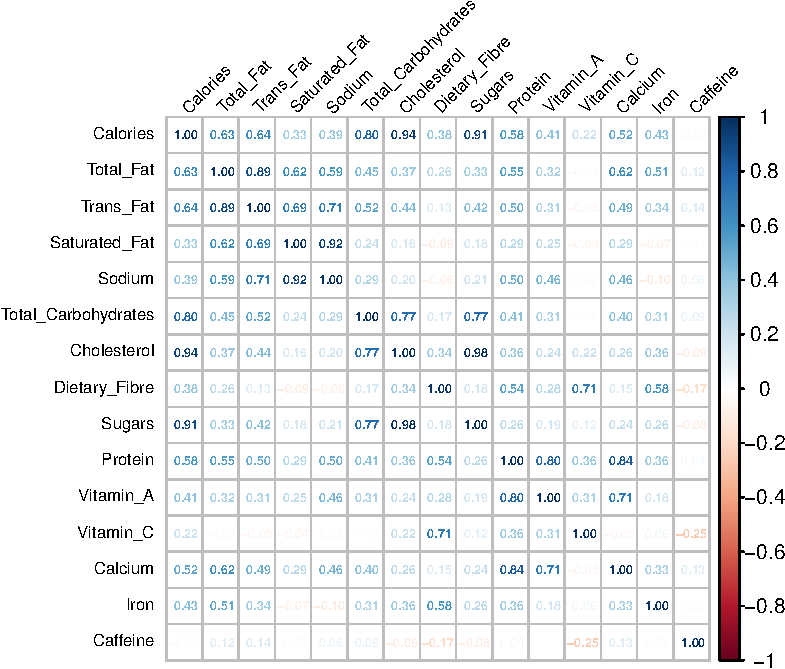
\includegraphics{Statistical_Learning_Final_Report_files/figure-latex/correlation_analysis-1} \end{center}

Moreover, we visualized the correlation matrix through a heatmap. The
heatmap provides a visual representation of the correlation matrix,
making it easier to identify patterns and relationships between the
variables. The color gradient helps to distinguish between positive and
negative correlations, with darker shades indicating stronger
correlations.

\begin{Shaded}
\begin{Highlighting}[]
\CommentTok{\# Heatmap of the correlation matrix}
\FunctionTok{heatmap}\NormalTok{(}\FunctionTok{cor}\NormalTok{(data\_num), }
        \AttributeTok{col =} \FunctionTok{colorRampPalette}\NormalTok{(}\FunctionTok{c}\NormalTok{(}\StringTok{"\#005cff"}\NormalTok{, }\StringTok{"\#fbfbfb"}\NormalTok{, }\StringTok{"\#d90000"}\NormalTok{))(}\DecValTok{100}\NormalTok{), }
        \AttributeTok{symm =} \ConstantTok{TRUE}\NormalTok{, }
        \AttributeTok{margins =} \FunctionTok{c}\NormalTok{(}\DecValTok{8}\NormalTok{, }\DecValTok{8}\NormalTok{), }
        \AttributeTok{cexRow =} \FloatTok{0.8}\NormalTok{,}
        \AttributeTok{cexCol =} \FloatTok{0.8}\NormalTok{)}
\end{Highlighting}
\end{Shaded}

\begin{center}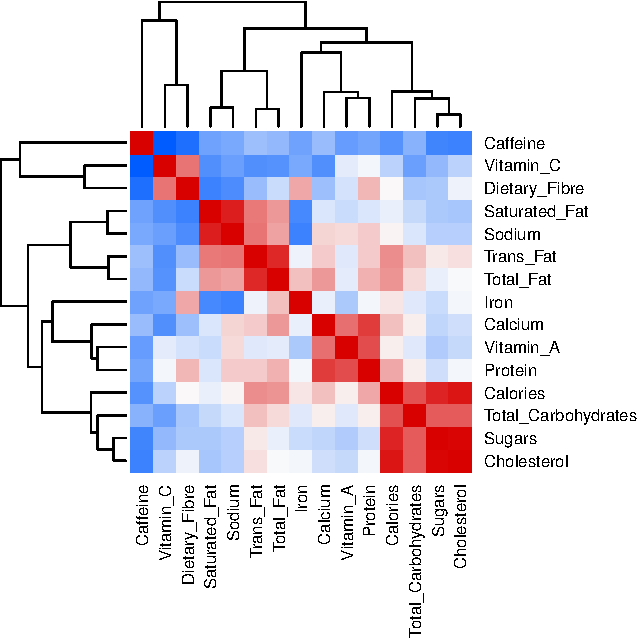
\includegraphics{Statistical_Learning_Final_Report_files/figure-latex/correlation_analysis_heatmap-1} \end{center}

\section{Data Visualization}\label{data-visualization}

\subsection{Histograms}\label{histograms}

We will plot some histograms to visualize the data.

\begin{Shaded}
\begin{Highlighting}[]
\CommentTok{\# Histogram of the data with density distribution}
\FunctionTok{par}\NormalTok{(}\AttributeTok{mfrow =} \FunctionTok{c}\NormalTok{(}\DecValTok{5}\NormalTok{, }\DecValTok{3}\NormalTok{), }\AttributeTok{mar =} \FunctionTok{c}\NormalTok{(}\DecValTok{2}\NormalTok{, }\DecValTok{2}\NormalTok{, }\DecValTok{2}\NormalTok{, }\DecValTok{2}\NormalTok{))}
\NormalTok{col }\OtherTok{\textless{}{-}} \FunctionTok{c}\NormalTok{(}\StringTok{\textquotesingle{}\#ff0000\textquotesingle{}}\NormalTok{, }\StringTok{\textquotesingle{}\#f70028\textquotesingle{}}\NormalTok{, }\StringTok{\textquotesingle{}\#ee0040\textquotesingle{}}\NormalTok{, }\StringTok{\textquotesingle{}\#e50055\textquotesingle{}}\NormalTok{, }\StringTok{\textquotesingle{}\#dc0069\textquotesingle{}}\NormalTok{,}
         \StringTok{\textquotesingle{}\#d2007b\textquotesingle{}}\NormalTok{, }\StringTok{\textquotesingle{}\#c7008d\textquotesingle{}}\NormalTok{, }\StringTok{\textquotesingle{}\#bb009e\textquotesingle{}}\NormalTok{, }\StringTok{\textquotesingle{}\#ae00ae\textquotesingle{}}\NormalTok{, }\StringTok{\textquotesingle{}\#a000be\textquotesingle{}}\NormalTok{,}
         \StringTok{\textquotesingle{}\#8f00cc\textquotesingle{}}\NormalTok{, }\StringTok{\textquotesingle{}\#7d00da\textquotesingle{}}\NormalTok{, }\StringTok{\textquotesingle{}\#6700e7\textquotesingle{}}\NormalTok{, }\StringTok{\textquotesingle{}\#4900f3\textquotesingle{}}\NormalTok{, }\StringTok{\textquotesingle{}\#0000ff\textquotesingle{}}\NormalTok{)}
\ControlFlowTok{for}\NormalTok{ (i }\ControlFlowTok{in} \DecValTok{1}\SpecialCharTok{:}\FunctionTok{ncol}\NormalTok{(data\_num)) \{}
  \FunctionTok{hist}\NormalTok{(data\_num[, i], }\AttributeTok{main =} \FunctionTok{colnames}\NormalTok{(data\_num)[i],}
       \AttributeTok{xlab =} \FunctionTok{colnames}\NormalTok{(data\_num)[i], }\AttributeTok{col =}\NormalTok{ col[i], }\AttributeTok{freq =} \ConstantTok{FALSE}\NormalTok{)}
\NormalTok{  dens }\OtherTok{\textless{}{-}} \FunctionTok{density}\NormalTok{(data\_num[, i], }\AttributeTok{na.rm=}\ConstantTok{TRUE}\NormalTok{, }\AttributeTok{adjust=}\FloatTok{1.25}\NormalTok{)}
  \FunctionTok{lines}\NormalTok{(dens, }\AttributeTok{col =} \StringTok{"black"}\NormalTok{, }\AttributeTok{lwd =} \DecValTok{2}\NormalTok{)}
\NormalTok{\}}
\end{Highlighting}
\end{Shaded}

\begin{center}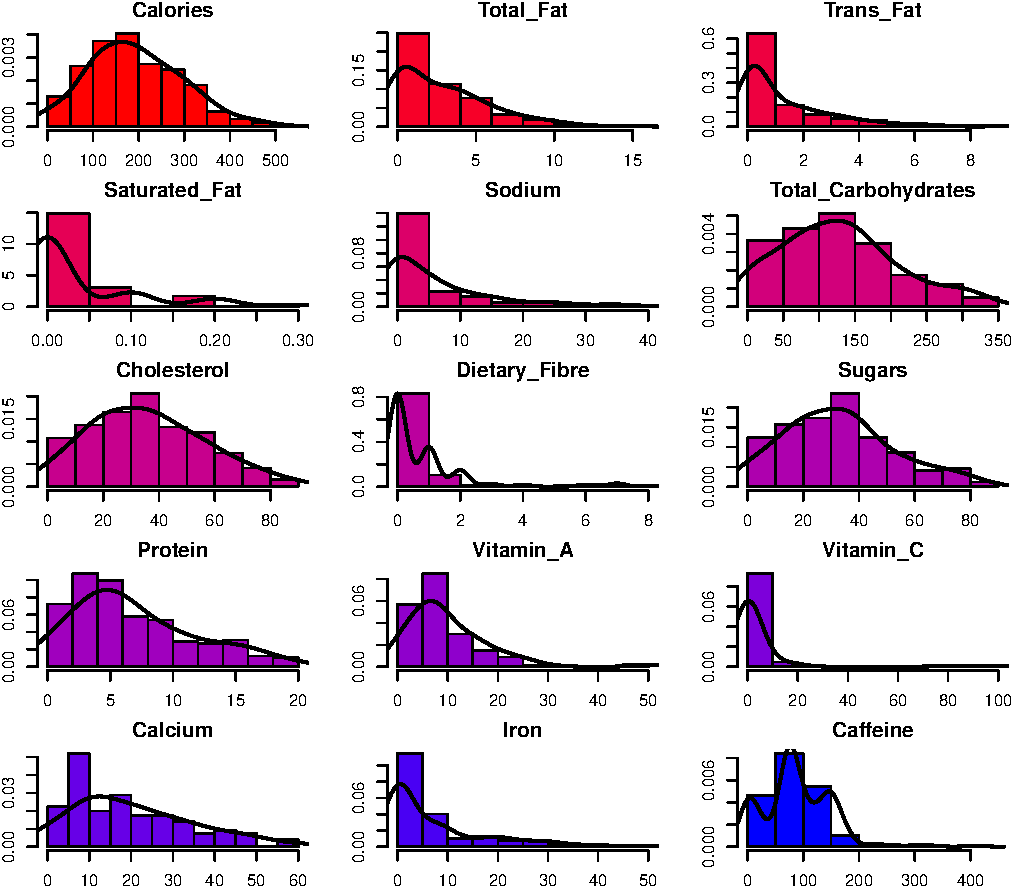
\includegraphics{Statistical_Learning_Final_Report_files/figure-latex/histograms-1} \end{center}

ADD COMMENTS ON THE GRAPH

\subsection{Pairplot}\label{pairplot}

We will plot a pairplot to visualize the relationship between the
variables. The pairplot is a grid of scatterplots that shows the
relationship between each pair of variables in the dataset. This
visualization helps us to identify patterns and correlations between the
variables.

First of all we have to define the function for the pairplot. We will
define a function for the histogram, the correlation and the smooth
line.

Then we create the pairplot using the defined functions.

\begin{Shaded}
\begin{Highlighting}[]
\FunctionTok{pairs}\NormalTok{(data\_num, }
      \AttributeTok{diag.panel =}\NormalTok{ panel.hist,}
      \AttributeTok{upper.panel =}\NormalTok{ panel.cor, }
      \AttributeTok{lower.panel =}\NormalTok{ panel.smooth,}
      \AttributeTok{colour =} \StringTok{"\#4ea5ff"}\NormalTok{)}
\end{Highlighting}
\end{Shaded}

\begin{center}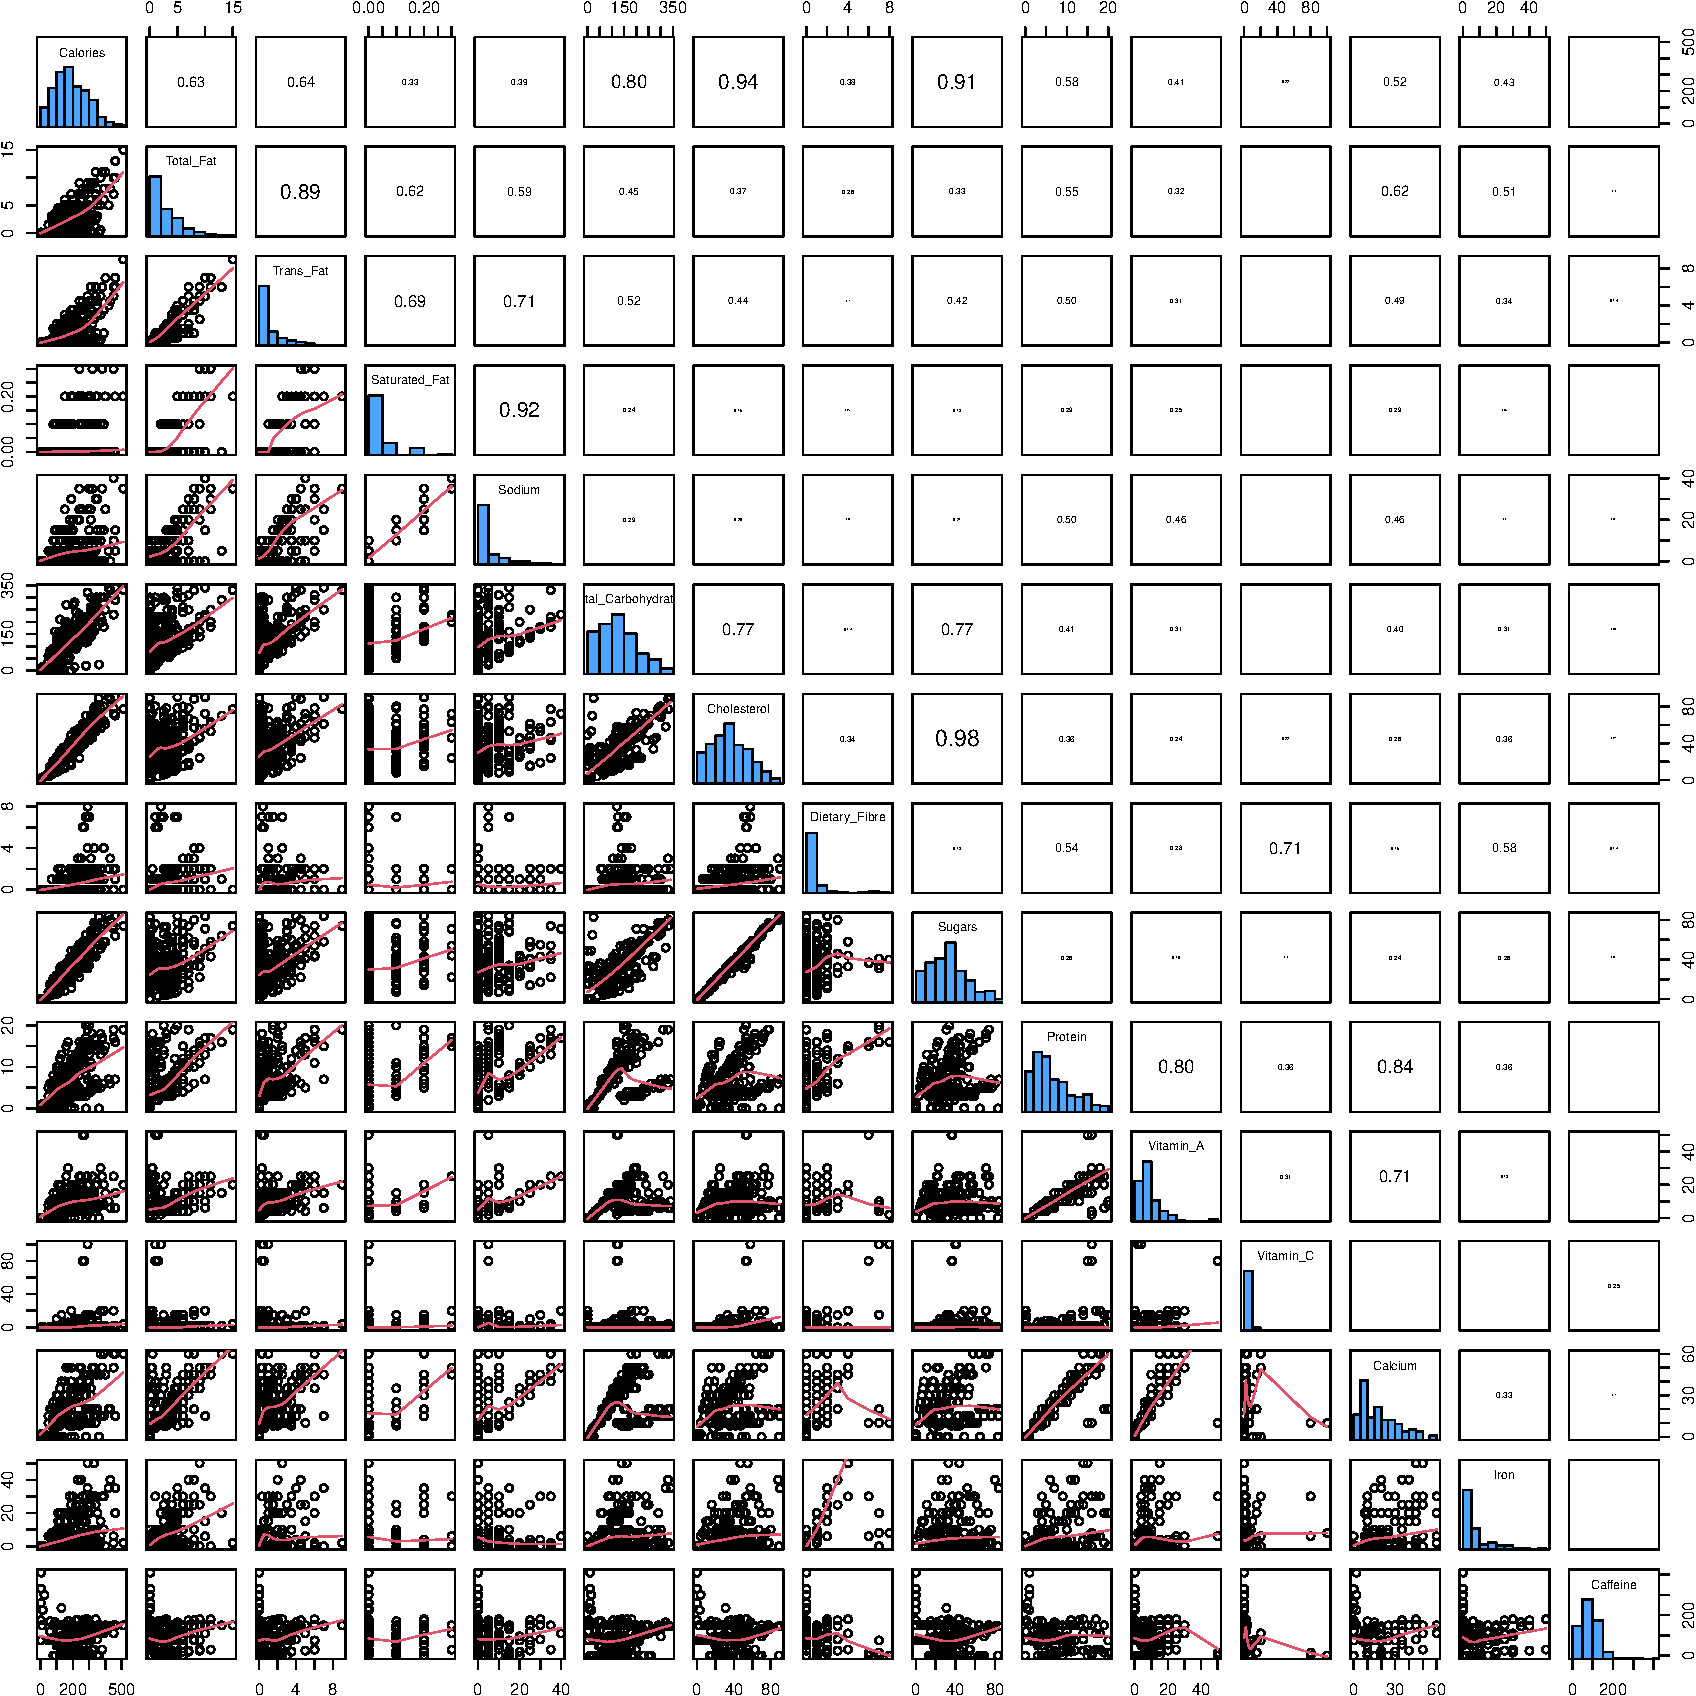
\includegraphics{Statistical_Learning_Final_Report_files/figure-latex/pairplot-1} \end{center}

ADD COMMENTS ON THE GRAPH

\subsection{Barplot}\label{barplot}

We will plot a barplot of the data. The barplot is a graphical
representation of the data that displays the frequency of each category
in a categorical variable. This visualization helps us to understand the
distribution of the data and identify the most common categories in the
dataset.

\begin{Shaded}
\begin{Highlighting}[]
\CommentTok{\# Barplot of the data}
\FunctionTok{par}\NormalTok{(}\AttributeTok{mfrow =} \FunctionTok{c}\NormalTok{(}\DecValTok{5}\NormalTok{, }\DecValTok{3}\NormalTok{), }\AttributeTok{mar =} \FunctionTok{c}\NormalTok{(}\DecValTok{2}\NormalTok{, }\DecValTok{2}\NormalTok{, }\DecValTok{2}\NormalTok{, }\DecValTok{2}\NormalTok{))}
\ControlFlowTok{for}\NormalTok{ (i }\ControlFlowTok{in} \DecValTok{1}\SpecialCharTok{:}\FunctionTok{ncol}\NormalTok{(data\_num)) \{}
  \FunctionTok{barplot}\NormalTok{(}\FunctionTok{table}\NormalTok{(data\_num[, i]), }\AttributeTok{main =} \FunctionTok{colnames}\NormalTok{(data\_num)[i],}
          \AttributeTok{xlab =} \FunctionTok{colnames}\NormalTok{(data\_num)[i], }\AttributeTok{col =}\NormalTok{ col[i], }\AttributeTok{border =}\NormalTok{ col[i])}
\NormalTok{\}}
\end{Highlighting}
\end{Shaded}

\begin{center}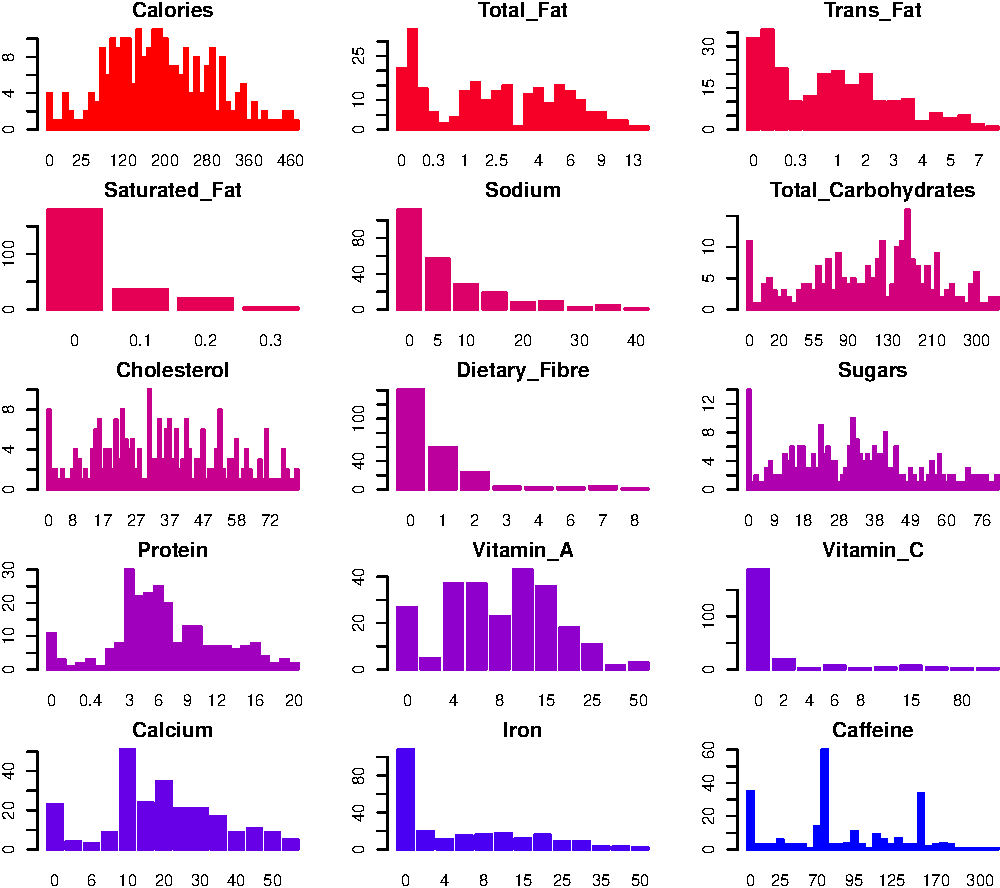
\includegraphics{Statistical_Learning_Final_Report_files/figure-latex/barplot-1} \end{center}

ADD COMMENTS ON THE GRAPH

\subsubsection{Beverages Barplot}\label{beverages-barplot}

We create a barplot to visualize the distribution of the
`Beverage\_category' variable and the `Beverage\_prep' variable in order
to understand the most common beverages and preparation methods.

\begin{Shaded}
\begin{Highlighting}[]
\CommentTok{\# Beverage category}
\FunctionTok{par}\NormalTok{(}\AttributeTok{mfrow =} \FunctionTok{c}\NormalTok{(}\DecValTok{1}\NormalTok{, }\DecValTok{1}\NormalTok{), }\AttributeTok{mar =} \FunctionTok{c}\NormalTok{(}\DecValTok{8}\NormalTok{, }\DecValTok{2}\NormalTok{, }\DecValTok{2}\NormalTok{, }\DecValTok{2}\NormalTok{))}
\FunctionTok{barplot}\NormalTok{(}\FunctionTok{table}\NormalTok{(data}\SpecialCharTok{$}\NormalTok{Beverage\_category),}
        \AttributeTok{main =} \StringTok{"Distribution of Beverage Categories"}\NormalTok{,}
        \AttributeTok{ylab =} \StringTok{"Count"}\NormalTok{,}
        \AttributeTok{col =} \StringTok{"\#4ea5ff"}\NormalTok{,}
        \AttributeTok{las =} \DecValTok{2}\NormalTok{, }
        \AttributeTok{cex.names =} \FloatTok{0.6}\NormalTok{)}
\end{Highlighting}
\end{Shaded}

\begin{center}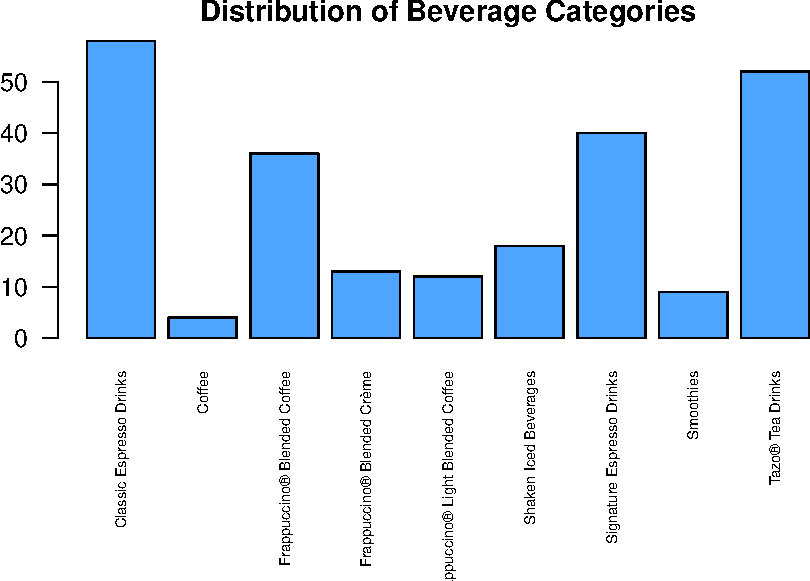
\includegraphics{Statistical_Learning_Final_Report_files/figure-latex/beverage_barplot-1} \end{center}

\begin{Shaded}
\begin{Highlighting}[]
\CommentTok{\# Beverage preparation}
\FunctionTok{barplot}\NormalTok{(}\FunctionTok{table}\NormalTok{(data}\SpecialCharTok{$}\NormalTok{Beverage\_prep),}
        \AttributeTok{main =} \StringTok{"Distribution of Beverage Preparation"}\NormalTok{,}
        \AttributeTok{ylab =} \StringTok{"Count"}\NormalTok{,}
        \AttributeTok{col =} \StringTok{"\#ff810f"}\NormalTok{,}
        \AttributeTok{las =} \DecValTok{2}\NormalTok{,}
        \AttributeTok{cex.names =} \FloatTok{0.6}\NormalTok{)}
\end{Highlighting}
\end{Shaded}

\begin{center}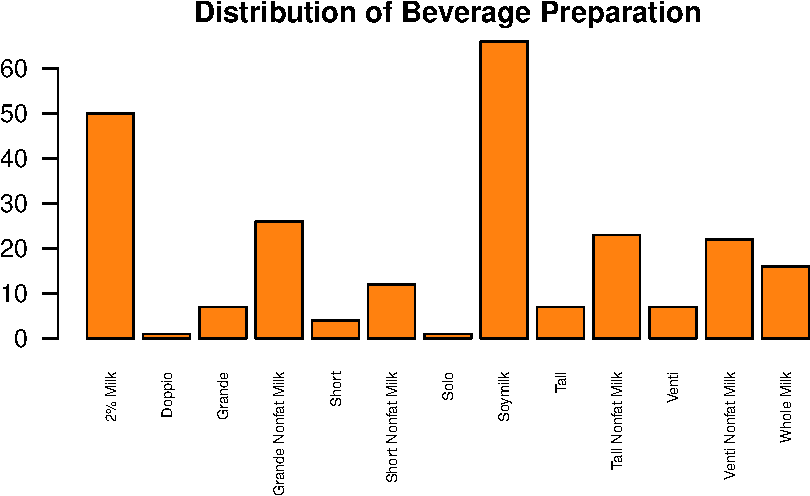
\includegraphics{Statistical_Learning_Final_Report_files/figure-latex/beverage_barplot-2} \end{center}

Now we want to compare the total calories for each categories of
bevarage. First we aggrgate the data to obtain the total calories for
each categories of bevarage and then we create a barplot to visualize
the results.

\begin{Shaded}
\begin{Highlighting}[]
\FunctionTok{par}\NormalTok{(}\AttributeTok{mfrow =} \FunctionTok{c}\NormalTok{(}\DecValTok{1}\NormalTok{, }\DecValTok{1}\NormalTok{), }\AttributeTok{mar =} \FunctionTok{c}\NormalTok{(}\DecValTok{8}\NormalTok{, }\DecValTok{2}\NormalTok{, }\DecValTok{2}\NormalTok{, }\DecValTok{2}\NormalTok{))}
\NormalTok{total\_calories\_by\_category }\OtherTok{\textless{}{-}} \FunctionTok{aggregate}\NormalTok{(Calories }\SpecialCharTok{\textasciitilde{}}\NormalTok{ Beverage\_category,}
                                        \AttributeTok{data =}\NormalTok{ data\_cleaned, sum)}

\FunctionTok{barplot}\NormalTok{(}\AttributeTok{height =}\NormalTok{ total\_calories\_by\_category}\SpecialCharTok{$}\NormalTok{Calories,}
        \AttributeTok{names.arg =}\NormalTok{ total\_calories\_by\_category}\SpecialCharTok{$}\NormalTok{Beverage\_category,}
        \AttributeTok{main =} \StringTok{"Total Calories by Beverage Category"}\NormalTok{,}
        \AttributeTok{ylab =} \StringTok{"Total Calories"}\NormalTok{,}
        \AttributeTok{col =} \StringTok{"\#4ea5ff"}\NormalTok{,}
        \AttributeTok{las =} \DecValTok{2}\NormalTok{,}
        \AttributeTok{cex.names =} \FloatTok{0.6}\NormalTok{)}
\end{Highlighting}
\end{Shaded}

\begin{center}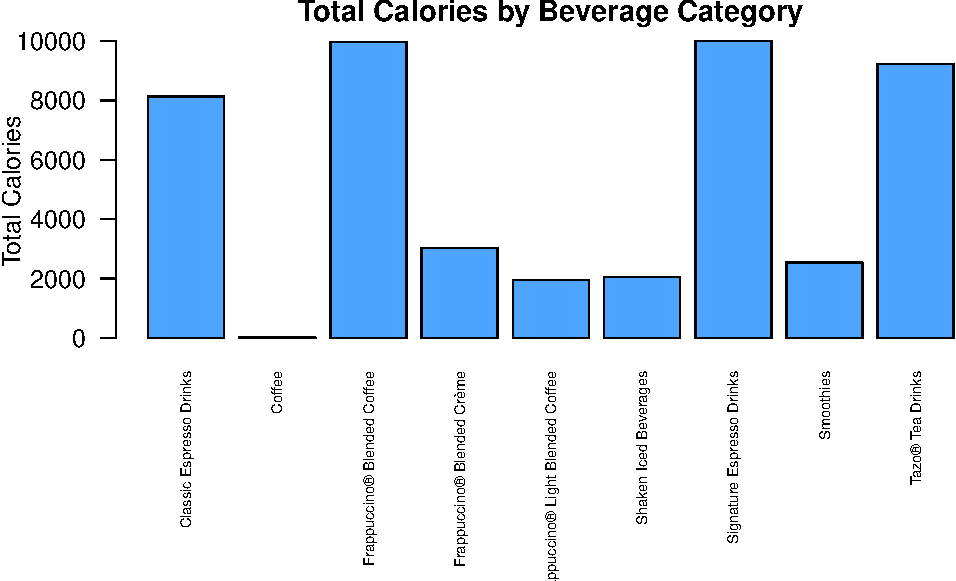
\includegraphics{Statistical_Learning_Final_Report_files/figure-latex/total_calories-1} \end{center}

Now we want to compare the total sugars for each preparation of
bevarage. First we aggrgate the data to obtain the total sugars for each
preparation of bevarage and then we create a barplot to visualize the
results.

\begin{Shaded}
\begin{Highlighting}[]
\FunctionTok{par}\NormalTok{(}\AttributeTok{mfrow =} \FunctionTok{c}\NormalTok{(}\DecValTok{1}\NormalTok{, }\DecValTok{1}\NormalTok{), }\AttributeTok{mar =} \FunctionTok{c}\NormalTok{(}\DecValTok{8}\NormalTok{, }\DecValTok{2}\NormalTok{, }\DecValTok{2}\NormalTok{, }\DecValTok{2}\NormalTok{))}
\NormalTok{total\_sugar\_by\_prep }\OtherTok{\textless{}{-}} \FunctionTok{aggregate}\NormalTok{(Total\_Carbohydrates }\SpecialCharTok{\textasciitilde{}}\NormalTok{ Beverage\_prep,}
                                 \AttributeTok{data =}\NormalTok{ data\_cleaned, sum)}

\FunctionTok{barplot}\NormalTok{(}\AttributeTok{height =}\NormalTok{ total\_sugar\_by\_prep}\SpecialCharTok{$}\NormalTok{Total\_Carbohydrates,}
        \AttributeTok{names.arg =}\NormalTok{ total\_sugar\_by\_prep}\SpecialCharTok{$}\NormalTok{Beverage\_prep,}
        \AttributeTok{main =} \StringTok{"Total Sugars by Beverage Preparation"}\NormalTok{,}
        \AttributeTok{ylab =} \StringTok{"Total Sugars (g)"}\NormalTok{,}
        \AttributeTok{col =} \StringTok{"\#ff810f"}\NormalTok{,}
        \AttributeTok{las =} \DecValTok{2}\NormalTok{,}
        \AttributeTok{cex.names =} \FloatTok{0.6}\NormalTok{)}
\end{Highlighting}
\end{Shaded}

\begin{center}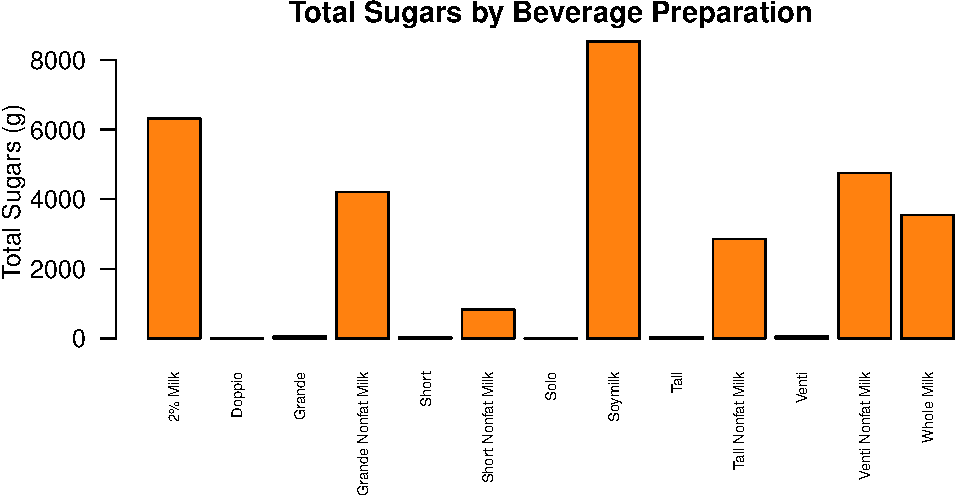
\includegraphics{Statistical_Learning_Final_Report_files/figure-latex/total_sugars-1} \end{center}

\subsection{Boxplot}\label{boxplot}

We will plot a boxplot of the data. The boxplot is a graphical
representation of the data that displays the distribution of the data,
including the median, quartiles, and outliers. This visualization helps
us to identify the spread and variability of the data.

\begin{Shaded}
\begin{Highlighting}[]
\CommentTok{\# Boxplot of the data}
\FunctionTok{par}\NormalTok{(}\AttributeTok{mfrow =} \FunctionTok{c}\NormalTok{(}\DecValTok{3}\NormalTok{, }\DecValTok{5}\NormalTok{), }\AttributeTok{mar =} \FunctionTok{c}\NormalTok{(}\DecValTok{2}\NormalTok{, }\DecValTok{2}\NormalTok{, }\DecValTok{2}\NormalTok{, }\DecValTok{2}\NormalTok{))}
\ControlFlowTok{for}\NormalTok{ (i }\ControlFlowTok{in} \DecValTok{1}\SpecialCharTok{:}\FunctionTok{ncol}\NormalTok{(data\_num)) \{}
  \FunctionTok{boxplot}\NormalTok{(data\_num[, i], }\AttributeTok{main =} \FunctionTok{colnames}\NormalTok{(data\_num)[i],}
          \AttributeTok{xlab =} \FunctionTok{colnames}\NormalTok{(data\_num)[i], }\AttributeTok{col =}\NormalTok{ col[i])}
\NormalTok{\}}
\end{Highlighting}
\end{Shaded}

\begin{center}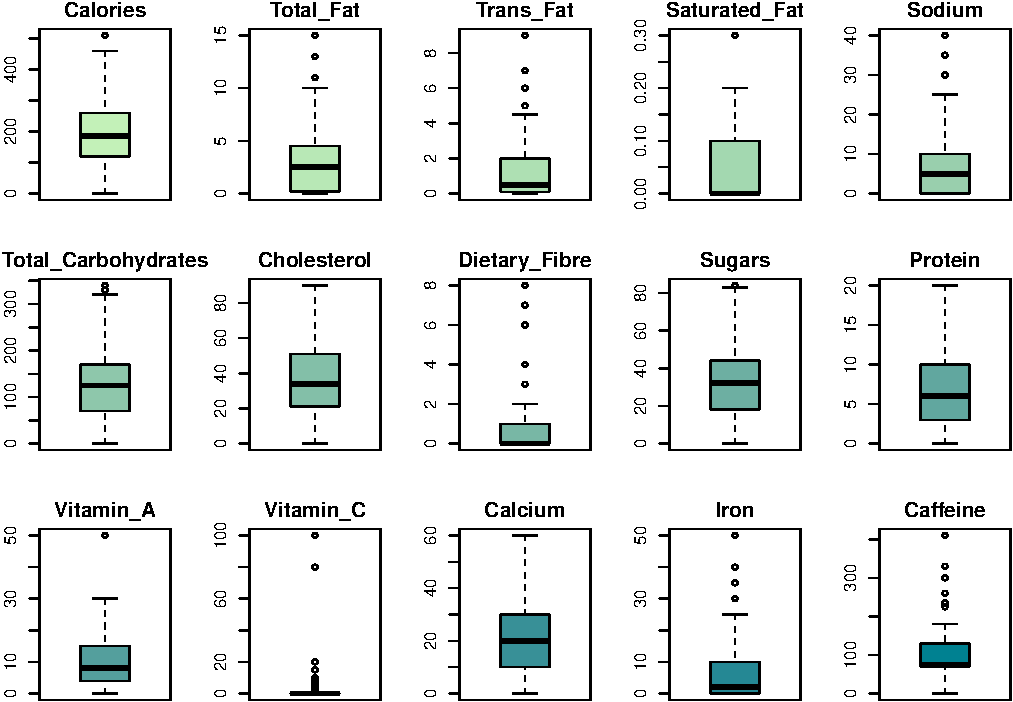
\includegraphics{Statistical_Learning_Final_Report_files/figure-latex/boxplot-1} \end{center}

\subsection{Scatterplot}\label{scatterplot}

We will plot a scatterplot of the data. The scatterplot is a graphical
representation of the data that displays the relationship between two
variables. This visualization helps us to identify patterns and
correlations between the variables.

We create a scatterplot to compare the amounts of calories and fat for
each categories of bevarage. We assign distinct colors to each beverage
category and create a legend to identify each category.

\begin{Shaded}
\begin{Highlighting}[]
\CommentTok{\# Set the variable as factor}
\NormalTok{data\_cleaned}\SpecialCharTok{$}\NormalTok{Beverage\_category }\OtherTok{\textless{}{-}} \FunctionTok{as.factor}\NormalTok{(data\_cleaned}\SpecialCharTok{$}\NormalTok{Beverage\_category)}

\CommentTok{\# Assign distinct colors to each beverage category}
\NormalTok{colors }\OtherTok{\textless{}{-}} \FunctionTok{rainbow}\NormalTok{(}\FunctionTok{length}\NormalTok{(}\FunctionTok{unique}\NormalTok{(data\_cleaned}\SpecialCharTok{$}\NormalTok{Beverage\_category)))}
\NormalTok{color\_map }\OtherTok{\textless{}{-}} \FunctionTok{setNames}\NormalTok{(colors, }\FunctionTok{levels}\NormalTok{(data\_cleaned}\SpecialCharTok{$}\NormalTok{Beverage\_category))}

\CommentTok{\# Create a scatterplot to compare amounts of calories and fat }
\CommentTok{\# for each categories of bevarage}
\FunctionTok{par}\NormalTok{(}\AttributeTok{mfrow =} \FunctionTok{c}\NormalTok{(}\DecValTok{1}\NormalTok{, }\DecValTok{1}\NormalTok{))}
\FunctionTok{plot}\NormalTok{(data\_cleaned}\SpecialCharTok{$}\NormalTok{Calories, }
\NormalTok{     data\_cleaned}\SpecialCharTok{$}\NormalTok{Total\_Fat\_g,}
     \AttributeTok{col =}\NormalTok{ color\_map[data\_cleaned}\SpecialCharTok{$}\NormalTok{Beverage\_category],}
     \AttributeTok{pch =} \DecValTok{19}\NormalTok{,}
     \AttributeTok{xlab =} \StringTok{"Calories"}\NormalTok{,}
     \AttributeTok{ylab =} \StringTok{"Total Fat (g)"}\NormalTok{,}
     \AttributeTok{main =} \StringTok{"Calories vs Total Fat"}\NormalTok{)}

\CommentTok{\# Legend}
\FunctionTok{legend}\NormalTok{(}\StringTok{"topleft"}\NormalTok{, }\AttributeTok{legend =} \FunctionTok{levels}\NormalTok{(data\_cleaned}\SpecialCharTok{$}\NormalTok{Beverage\_category), }
       \AttributeTok{col =}\NormalTok{ colors, }\AttributeTok{cex =} \FloatTok{0.4}\NormalTok{, }\AttributeTok{pch =} \DecValTok{19}\NormalTok{)}
\end{Highlighting}
\end{Shaded}

\begin{center}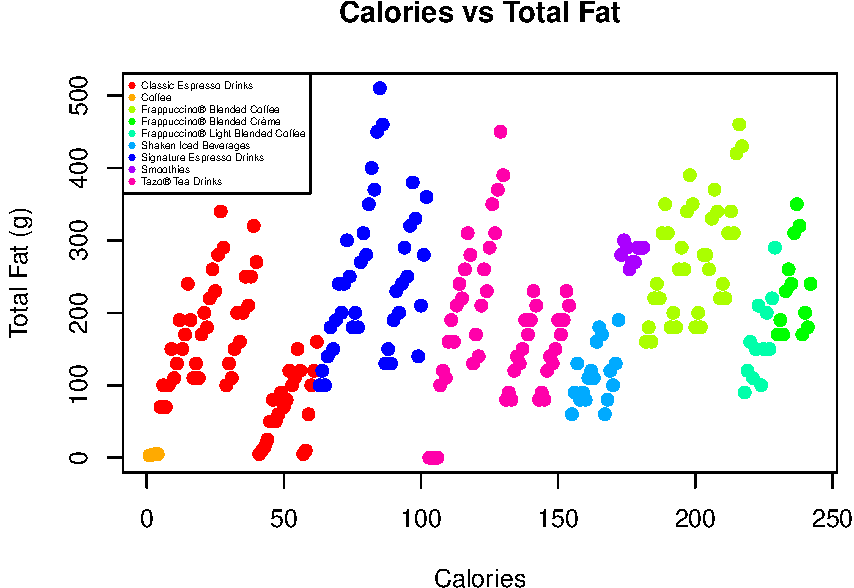
\includegraphics{Statistical_Learning_Final_Report_files/figure-latex/fat_comparison-1} \end{center}

\begin{Shaded}
\begin{Highlighting}[]
\CommentTok{\# Comparision between total fat and trans fat ( che cazzo sono?)}

\CommentTok{\# Numeric variable {-}\textgreater{} calculate density}
\NormalTok{total\_fat\_density }\OtherTok{\textless{}{-}} \FunctionTok{density}\NormalTok{(data\_cleaned}\SpecialCharTok{$}\NormalTok{Total\_Fat)}
\NormalTok{trans\_fat\_density }\OtherTok{\textless{}{-}} \FunctionTok{density}\NormalTok{(data\_cleaned}\SpecialCharTok{$}\NormalTok{Trans\_Fat)}

\FunctionTok{plot}\NormalTok{(total\_fat\_density, }\AttributeTok{col =} \StringTok{"\#4ea5ff"}\NormalTok{,}
     \AttributeTok{main =} \StringTok{"Comparison of Total Fat and Trans Fat Distributions"}\NormalTok{, }
     \AttributeTok{xlab =} \StringTok{"Fat Content (g)"}\NormalTok{, }\AttributeTok{ylab =} \StringTok{"Density"}\NormalTok{, }
     \AttributeTok{ylim =} \FunctionTok{c}\NormalTok{(}\DecValTok{0}\NormalTok{, }\FunctionTok{max}\NormalTok{(total\_fat\_density}\SpecialCharTok{$}\NormalTok{y, trans\_fat\_density}\SpecialCharTok{$}\NormalTok{y)),}
     \AttributeTok{xlim =} \FunctionTok{range}\NormalTok{(data\_cleaned}\SpecialCharTok{$}\NormalTok{Total\_Fat, data\_cleaned}\SpecialCharTok{$}\NormalTok{Trans\_Fat), }
     \AttributeTok{lwd =} \DecValTok{2}\NormalTok{, }\AttributeTok{lty =} \DecValTok{1}\NormalTok{)}
\FunctionTok{lines}\NormalTok{(trans\_fat\_density, }\AttributeTok{col =} \StringTok{"\#ff810f"}\NormalTok{, }\AttributeTok{lwd =} \DecValTok{2}\NormalTok{, }\AttributeTok{lty =} \DecValTok{1}\NormalTok{)}
\FunctionTok{legend}\NormalTok{(}\StringTok{"topright"}\NormalTok{, }\AttributeTok{legend =} \FunctionTok{c}\NormalTok{(}\StringTok{"Total Fat"}\NormalTok{, }\StringTok{"Trans Fat"}\NormalTok{),}
       \AttributeTok{col =} \FunctionTok{c}\NormalTok{(}\StringTok{"\#4ea5ff"}\NormalTok{, }\StringTok{"\#ff810f"}\NormalTok{), }\AttributeTok{lwd =} \DecValTok{2}\NormalTok{, }\AttributeTok{lty =} \DecValTok{1}\NormalTok{)}
\end{Highlighting}
\end{Shaded}

\begin{center}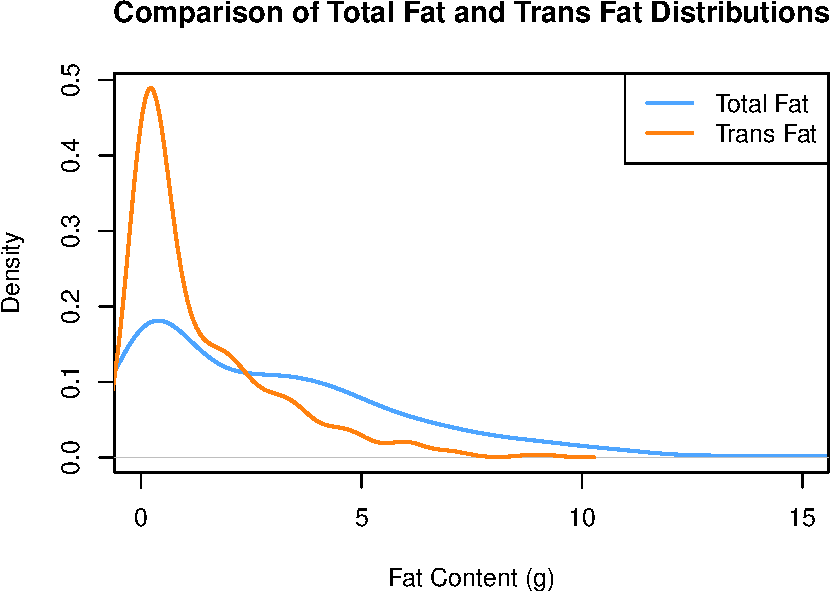
\includegraphics{Statistical_Learning_Final_Report_files/figure-latex/fat_comparison-2} \end{center}

Create scatterplot to look into relantionship between calories and other
variables. We will plot the relationship between calories and sodium,
protein, vitamin C and fiber.

\begin{Shaded}
\begin{Highlighting}[]
\FunctionTok{par}\NormalTok{(}\AttributeTok{mfrow =} \FunctionTok{c}\NormalTok{(}\DecValTok{2}\NormalTok{, }\DecValTok{2}\NormalTok{), }\AttributeTok{mar =} \FunctionTok{c}\NormalTok{(}\DecValTok{4}\NormalTok{, }\DecValTok{4}\NormalTok{, }\DecValTok{2}\NormalTok{, }\DecValTok{2}\NormalTok{))}
\FunctionTok{with}\NormalTok{(data\_cleaned, \{}
  \FunctionTok{plot}\NormalTok{(Calories, Sodium , }\AttributeTok{main =} \StringTok{"Relation between Calories and Sodium"}\NormalTok{,}
       \AttributeTok{xlab =} \StringTok{"Calories"}\NormalTok{, }\AttributeTok{ylab =} \StringTok{"Sodium (mg)"}\NormalTok{, }\AttributeTok{col =}\NormalTok{ col[}\DecValTok{1}\NormalTok{])}
  \FunctionTok{plot}\NormalTok{(Calories, Protein , }\AttributeTok{main =} \StringTok{"Relation between Calories and Protein"}\NormalTok{,}
       \AttributeTok{xlab =} \StringTok{"Calories"}\NormalTok{, }\AttributeTok{ylab =} \StringTok{"Protein (g)"}\NormalTok{, }\AttributeTok{col =}\NormalTok{ col[}\DecValTok{5}\NormalTok{])}
  \FunctionTok{plot}\NormalTok{(Calories, Vitamin\_C , }\AttributeTok{main =} \StringTok{"Relation between Calories and Vitamin C"}\NormalTok{,}
       \AttributeTok{xlab =} \StringTok{"Calories"}\NormalTok{, }\AttributeTok{ylab =} \StringTok{"Vitamin C (mg)"}\NormalTok{, }\AttributeTok{col =}\NormalTok{ col[}\DecValTok{10}\NormalTok{])}
  \FunctionTok{plot}\NormalTok{(Calories, Cholesterol , }\AttributeTok{main =} \StringTok{"Relation between Calories and Fiber"}\NormalTok{,}
       \AttributeTok{xlab =} \StringTok{"Calories"}\NormalTok{, }\AttributeTok{ylab =} \StringTok{"Fiber (g)"}\NormalTok{, }\AttributeTok{col =}\NormalTok{ col[}\DecValTok{15}\NormalTok{])}
\NormalTok{\})}
\end{Highlighting}
\end{Shaded}

\begin{center}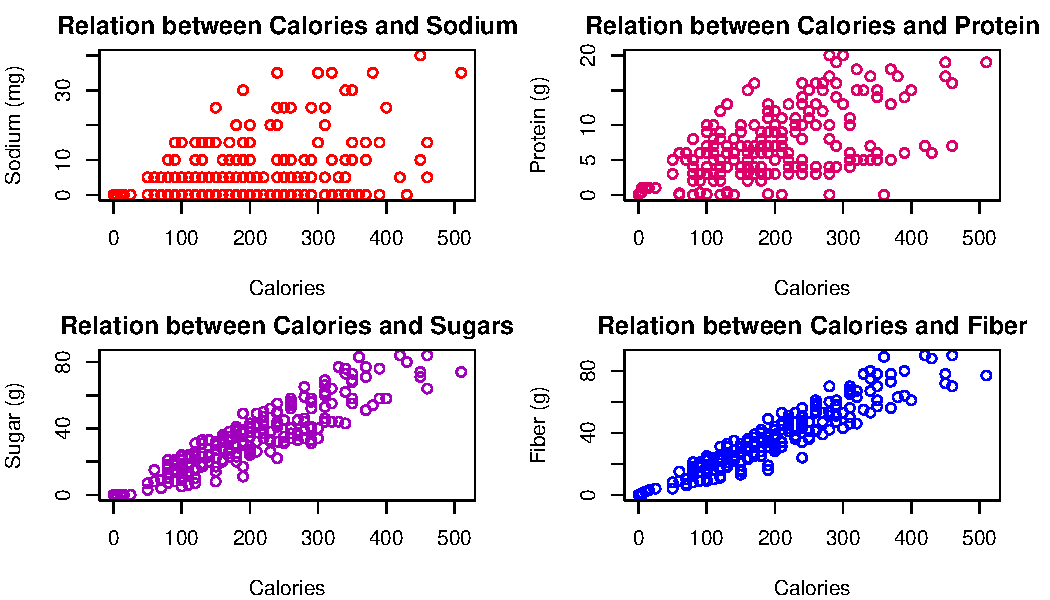
\includegraphics{Statistical_Learning_Final_Report_files/figure-latex/scatterplot-1} \end{center}

There's increase in every feature with increase in calories. Features
like proteins and fiber rapidly increase, instead vitamin and
cholesterol more flat growing. Confirmed by correlation coefficients

ADD COMMENTS ON THE GRAPH

\section{Regression Analysis}\label{regression-analysis}

\subsection{Linear Regression}\label{linear-regression}

Linear regression model to predict the amount of calories based on the
amount of the other variables We use the lm() function to fit a linear
regression model

\begin{Shaded}
\begin{Highlighting}[]
\CommentTok{\# Fit the linear regression model}

\CommentTok{\# Set the calories as the dependent variable}
\NormalTok{y }\OtherTok{\textless{}{-}}\NormalTok{ data\_num}\SpecialCharTok{$}\NormalTok{Calories}

\CommentTok{\# Remove calories column in order to use the other variables }
\CommentTok{\# as independent variables}
\NormalTok{data\_num }\OtherTok{\textless{}{-}}\NormalTok{ data\_num[, }\SpecialCharTok{{-}}\DecValTok{1}\NormalTok{]}

\NormalTok{lm\_model }\OtherTok{\textless{}{-}} \FunctionTok{lm}\NormalTok{(y }\SpecialCharTok{\textasciitilde{}}\NormalTok{ ., }\AttributeTok{data =}\NormalTok{ data\_num)}
\FunctionTok{summary}\NormalTok{(lm\_model)}
\end{Highlighting}
\end{Shaded}

\begin{verbatim}
## 
## Call:
## lm(formula = y ~ ., data = data_num)
## 
## Residuals:
##      Min       1Q   Median       3Q      Max 
## -14.0233  -3.3009  -0.3806   3.0039  21.9404 
## 
## Coefficients:
##                      Estimate Std. Error t value Pr(>|t|)    
## (Intercept)          0.252316   0.952833   0.265  0.79140    
## Total_Fat           11.143733   0.532812  20.915  < 2e-16 ***
## Trans_Fat           -2.477820   0.809270  -3.062  0.00247 ** 
## Saturated_Fat       -9.816317  18.143619  -0.541  0.58901    
## Sodium              -0.279257   0.167487  -1.667  0.09683 .  
## Total_Carbohydrates  0.020972   0.007420   2.826  0.00513 ** 
## Cholesterol          2.829543   0.340268   8.316 8.43e-15 ***
## Dietary_Fibre        1.534913   0.942106   1.629  0.10465    
## Sugars               1.131045   0.348234   3.248  0.00134 ** 
## Protein              2.218895   0.510445   4.347 2.08e-05 ***
## Vitamin_A            0.162307   0.083662   1.940  0.05361 .  
## Vitamin_C            0.147669   0.047675   3.097  0.00220 ** 
## Calcium              0.462193   0.142257   3.249  0.00133 ** 
## Iron                -0.649101   0.070666  -9.185  < 2e-16 ***
## Caffeine             0.013513   0.005826   2.319  0.02126 *  
## ---
## Signif. codes:  0 '***' 0.001 '**' 0.01 '*' 0.05 '.' 0.1 ' ' 1
## 
## Residual standard error: 5.126 on 227 degrees of freedom
## Multiple R-squared:  0.9977, Adjusted R-squared:  0.9975 
## F-statistic:  6915 on 14 and 227 DF,  p-value: < 2.2e-16
\end{verbatim}

\begin{Shaded}
\begin{Highlighting}[]
\FunctionTok{par}\NormalTok{(}\AttributeTok{mfrow =} \FunctionTok{c}\NormalTok{(}\DecValTok{2}\NormalTok{, }\DecValTok{2}\NormalTok{), }\AttributeTok{mar =} \FunctionTok{c}\NormalTok{(}\DecValTok{2}\NormalTok{, }\DecValTok{2}\NormalTok{, }\DecValTok{2}\NormalTok{, }\DecValTok{2}\NormalTok{))}
\FunctionTok{plot}\NormalTok{(lm\_model)}
\end{Highlighting}
\end{Shaded}

\begin{center}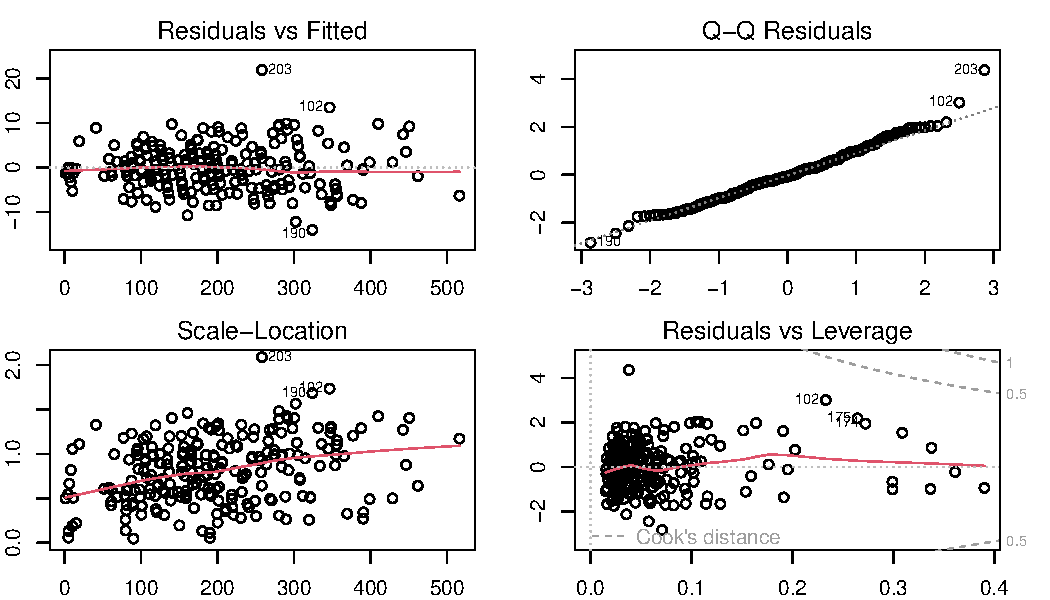
\includegraphics{Statistical_Learning_Final_Report_files/figure-latex/linear_regression-1} \end{center}

\begin{Shaded}
\begin{Highlighting}[]
\FunctionTok{AIC}\NormalTok{(lm\_model)}
\end{Highlighting}
\end{Shaded}

\begin{verbatim}
## [1] 1494.304
\end{verbatim}

\begin{Shaded}
\begin{Highlighting}[]
\FunctionTok{BIC}\NormalTok{(lm\_model)}
\end{Highlighting}
\end{Shaded}

\begin{verbatim}
## [1] 1550.127
\end{verbatim}

The model has a low AIC and BIC values, the R-squared value is 0.99 so
the model is a good fit for the data. The model is significant, the
p-value is less than 0.05

\subsection{Logistic Regression}\label{logistic-regression}

Logistic regression model to predict the amount of calories based on the
amount of the other variables We use the glm() function to fit a
logistic regression model

\begin{Shaded}
\begin{Highlighting}[]
\CommentTok{\# Fit the logistic regression model}

\NormalTok{glm\_model }\OtherTok{\textless{}{-}} \FunctionTok{glm}\NormalTok{(y }\SpecialCharTok{\textasciitilde{}}\NormalTok{ ., }\AttributeTok{data =}\NormalTok{ data\_num, }\AttributeTok{family =} \StringTok{"gaussian"}\NormalTok{) }
\CommentTok{\# Try to change the family}
\FunctionTok{summary}\NormalTok{(glm\_model)}
\end{Highlighting}
\end{Shaded}

\begin{verbatim}
## 
## Call:
## glm(formula = y ~ ., family = "gaussian", data = data_num)
## 
## Coefficients:
##                      Estimate Std. Error t value Pr(>|t|)    
## (Intercept)          0.252316   0.952833   0.265  0.79140    
## Total_Fat           11.143733   0.532812  20.915  < 2e-16 ***
## Trans_Fat           -2.477820   0.809270  -3.062  0.00247 ** 
## Saturated_Fat       -9.816317  18.143619  -0.541  0.58901    
## Sodium              -0.279257   0.167487  -1.667  0.09683 .  
## Total_Carbohydrates  0.020972   0.007420   2.826  0.00513 ** 
## Cholesterol          2.829543   0.340268   8.316 8.43e-15 ***
## Dietary_Fibre        1.534913   0.942106   1.629  0.10465    
## Sugars               1.131045   0.348234   3.248  0.00134 ** 
## Protein              2.218895   0.510445   4.347 2.08e-05 ***
## Vitamin_A            0.162307   0.083662   1.940  0.05361 .  
## Vitamin_C            0.147669   0.047675   3.097  0.00220 ** 
## Calcium              0.462193   0.142257   3.249  0.00133 ** 
## Iron                -0.649101   0.070666  -9.185  < 2e-16 ***
## Caffeine             0.013513   0.005826   2.319  0.02126 *  
## ---
## Signif. codes:  0 '***' 0.001 '**' 0.01 '*' 0.05 '.' 0.1 ' ' 1
## 
## (Dispersion parameter for gaussian family taken to be 26.27685)
## 
##     Null deviance: 2549987.0  on 241  degrees of freedom
## Residual deviance:    5964.8  on 227  degrees of freedom
## AIC: 1494.3
## 
## Number of Fisher Scoring iterations: 2
\end{verbatim}

\begin{Shaded}
\begin{Highlighting}[]
\FunctionTok{par}\NormalTok{(}\AttributeTok{mfrow =} \FunctionTok{c}\NormalTok{(}\DecValTok{2}\NormalTok{, }\DecValTok{2}\NormalTok{), }\AttributeTok{mar =} \FunctionTok{c}\NormalTok{(}\DecValTok{2}\NormalTok{, }\DecValTok{2}\NormalTok{, }\DecValTok{2}\NormalTok{, }\DecValTok{2}\NormalTok{))}
\FunctionTok{plot}\NormalTok{(glm\_model)}
\end{Highlighting}
\end{Shaded}

\begin{center}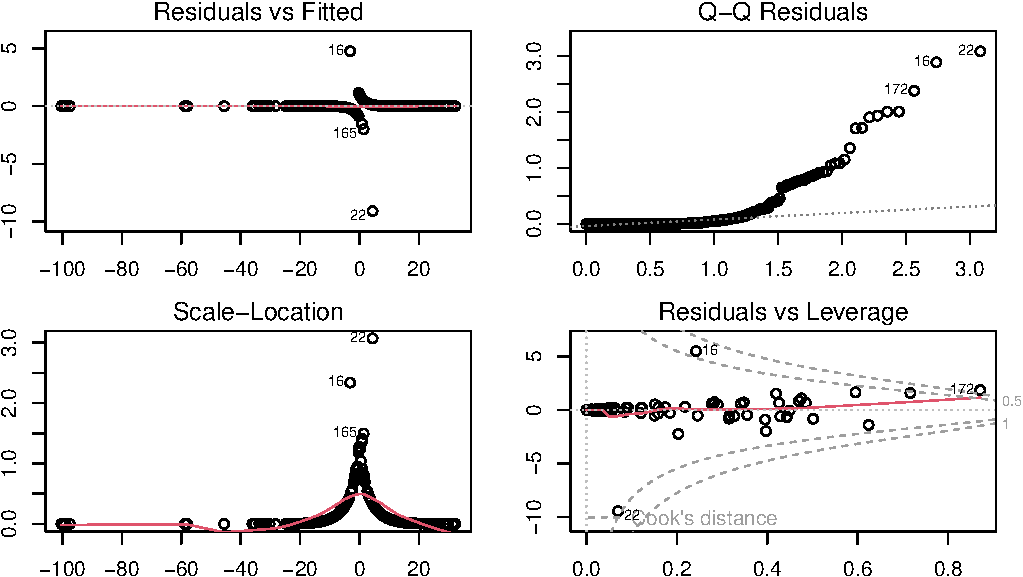
\includegraphics{Statistical_Learning_Final_Report_files/figure-latex/logistic_regression-1} \end{center}

\begin{Shaded}
\begin{Highlighting}[]
\FunctionTok{AIC}\NormalTok{(glm\_model)}
\end{Highlighting}
\end{Shaded}

\begin{verbatim}
## [1] 1494.304
\end{verbatim}

\begin{Shaded}
\begin{Highlighting}[]
\FunctionTok{BIC}\NormalTok{(glm\_model)}
\end{Highlighting}
\end{Shaded}

\begin{verbatim}
## [1] 1550.127
\end{verbatim}

\subsection{Cross Validation}\label{cross-validation}

Cross validation is a technique used to evaluate the performance of a
model. It involves splitting the data into training and testing sets,
fitting the model using the training set, and evaluating the model using
the testing set. This process is repeated multiple times to ensure that
the model is robust and generalizes well to new data.

\subsubsection{Linear Regression}\label{linear-regression-1}

We split the data into training and testing sets, fit the linear
regression model using the training set.

\begin{Shaded}
\begin{Highlighting}[]
\CommentTok{\# Split the data into training and testing sets}
\FunctionTok{set.seed}\NormalTok{(}\DecValTok{123}\NormalTok{)}
\NormalTok{train\_index }\OtherTok{\textless{}{-}} \FunctionTok{sample}\NormalTok{(}\DecValTok{1}\SpecialCharTok{:}\FunctionTok{nrow}\NormalTok{(data\_num), }\FloatTok{0.8} \SpecialCharTok{*} \FunctionTok{nrow}\NormalTok{(data\_num))}
\NormalTok{train\_data }\OtherTok{\textless{}{-}}\NormalTok{ data\_num[train\_index, ]}
\NormalTok{test\_data }\OtherTok{\textless{}{-}}\NormalTok{ data\_num[}\SpecialCharTok{{-}}\NormalTok{train\_index, ]}

\CommentTok{\# Fit the linear regression model using the training set}
\NormalTok{y\_train }\OtherTok{\textless{}{-}}\NormalTok{ y[train\_index]}

\NormalTok{lm\_model\_train }\OtherTok{\textless{}{-}} \FunctionTok{lm}\NormalTok{(y\_train }\SpecialCharTok{\textasciitilde{}}\NormalTok{ ., }\AttributeTok{data =}\NormalTok{ train\_data)}
\FunctionTok{summary}\NormalTok{(lm\_model\_train)}
\end{Highlighting}
\end{Shaded}

\begin{verbatim}
## 
## Call:
## lm(formula = y_train ~ ., data = train_data)
## 
## Residuals:
##      Min       1Q   Median       3Q      Max 
## -13.3660  -3.4895  -0.3014   3.2957  22.0511 
## 
## Coefficients:
##                      Estimate Std. Error t value Pr(>|t|)    
## (Intercept)          0.384009   1.086638   0.353 0.724213    
## Total_Fat           11.010780   0.584930  18.824  < 2e-16 ***
## Trans_Fat           -2.384286   0.926402  -2.574 0.010876 *  
## Saturated_Fat       -6.394565  19.670475  -0.325 0.745499    
## Sodium              -0.344189   0.189423  -1.817 0.070894 .  
## Total_Carbohydrates  0.018919   0.008550   2.213 0.028182 *  
## Cholesterol          2.688521   0.393449   6.833 1.27e-10 ***
## Dietary_Fibre        1.334079   1.068310   1.249 0.213387    
## Sugars               1.270177   0.402629   3.155 0.001886 ** 
## Protein              2.288347   0.598184   3.825 0.000180 ***
## Vitamin_A            0.153517   0.104811   1.465 0.144767    
## Vitamin_C            0.192040   0.055413   3.466 0.000663 ***
## Calcium              0.458855   0.163646   2.804 0.005609 ** 
## Iron                -0.571726   0.080401  -7.111 2.70e-11 ***
## Caffeine             0.016253   0.006917   2.350 0.019895 *  
## ---
## Signif. codes:  0 '***' 0.001 '**' 0.01 '*' 0.05 '.' 0.1 ' ' 1
## 
## Residual standard error: 5.168 on 178 degrees of freedom
## Multiple R-squared:  0.9975, Adjusted R-squared:  0.9973 
## F-statistic:  5061 on 14 and 178 DF,  p-value: < 2.2e-16
\end{verbatim}

\begin{Shaded}
\begin{Highlighting}[]
\FunctionTok{AIC}\NormalTok{(lm\_model\_train)}
\end{Highlighting}
\end{Shaded}

\begin{verbatim}
## [1] 1198.059
\end{verbatim}

\begin{Shaded}
\begin{Highlighting}[]
\FunctionTok{BIC}\NormalTok{(lm\_model\_train)}
\end{Highlighting}
\end{Shaded}

\begin{verbatim}
## [1] 1250.262
\end{verbatim}

\paragraph{Model Evaluation}\label{model-evaluation}

We evaluate the model using the testing set. We make predictions using
the testing set and calculate the mean squared error and the root mean
squared error to assess the model's accuracy. We also plot the residuals
to check if the model is a good fit.

\begin{Shaded}
\begin{Highlighting}[]
\CommentTok{\# Make predictions using the testing set}
\NormalTok{y\_test }\OtherTok{\textless{}{-}}\NormalTok{ y[}\SpecialCharTok{{-}}\NormalTok{train\_index]}
\NormalTok{predictions\_lm }\OtherTok{\textless{}{-}} \FunctionTok{predict}\NormalTok{(lm\_model\_train, }\AttributeTok{newdata =}\NormalTok{ test\_data)}

\CommentTok{\# Evaluate the model using the testing set}

\CommentTok{\# Calculate the mean squared error}
\NormalTok{mse\_lm}\OtherTok{\textless{}{-}} \FunctionTok{mean}\NormalTok{((y\_test }\SpecialCharTok{{-}}\NormalTok{ predictions\_lm)}\SpecialCharTok{\^{}}\DecValTok{2}\NormalTok{)}
\NormalTok{mse\_lm}
\end{Highlighting}
\end{Shaded}

\begin{verbatim}
## [1] 27.00986
\end{verbatim}

\begin{Shaded}
\begin{Highlighting}[]
\CommentTok{\# Calculate the root mean squared error}
\NormalTok{rmse\_lm }\OtherTok{\textless{}{-}} \FunctionTok{sqrt}\NormalTok{(mse\_lm)}
\NormalTok{rmse\_lm}
\end{Highlighting}
\end{Shaded}

\begin{verbatim}
## [1] 5.197101
\end{verbatim}

\begin{Shaded}
\begin{Highlighting}[]
\CommentTok{\# Now we plot the residuals to check if the model is a good fit}
\FunctionTok{par}\NormalTok{(}\AttributeTok{mfrow =} \FunctionTok{c}\NormalTok{(}\DecValTok{1}\NormalTok{, }\DecValTok{1}\NormalTok{))}
\FunctionTok{plot}\NormalTok{(lm\_model\_train, }\AttributeTok{which =} \DecValTok{1}\NormalTok{)}
\end{Highlighting}
\end{Shaded}

\begin{center}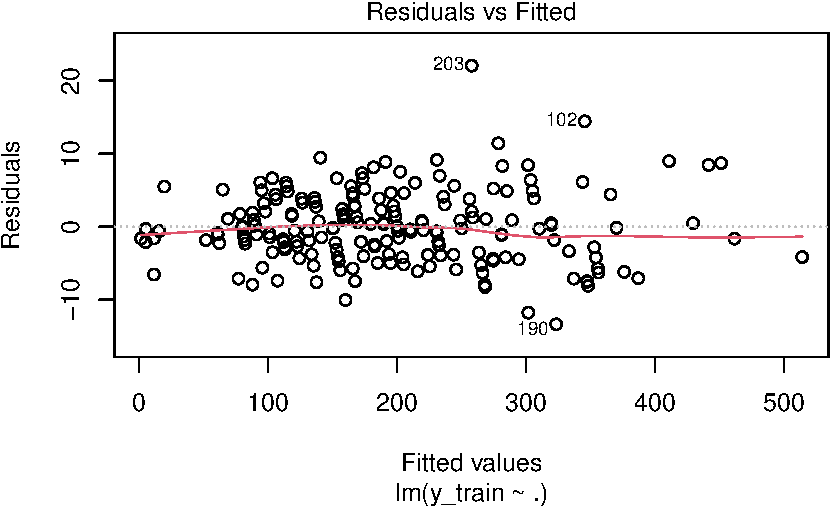
\includegraphics{Statistical_Learning_Final_Report_files/figure-latex/model_evaluation_lm-1} \end{center}

The residuals are randomly distributed around zero, so the model is a
good fit

Now we compute the accuracy of the model and then we plot the results

\begin{Shaded}
\begin{Highlighting}[]
\CommentTok{\# Compute the accuracy of the model}
\NormalTok{accuracy\_lm }\OtherTok{\textless{}{-}} \DecValTok{1} \SpecialCharTok{{-}}\NormalTok{ (rmse\_lm }\SpecialCharTok{/} \FunctionTok{mean}\NormalTok{(y\_test))}
\NormalTok{accuracy\_lm}
\end{Highlighting}
\end{Shaded}

\begin{verbatim}
## [1] 0.972211
\end{verbatim}

\begin{Shaded}
\begin{Highlighting}[]
\CommentTok{\# Plot the results}
\FunctionTok{plot}\NormalTok{(y\_test, predictions\_lm, }\AttributeTok{main =} \StringTok{"Actual vs Predicted Values"}\NormalTok{,}
     \AttributeTok{xlab =} \StringTok{"Actual Values"}\NormalTok{, }\AttributeTok{ylab =} \StringTok{"Predicted Values"}\NormalTok{,}
     \AttributeTok{col =} \StringTok{"\#4ea5ff"}\NormalTok{, }\AttributeTok{pch =} \DecValTok{19}\NormalTok{)}
\end{Highlighting}
\end{Shaded}

\begin{center}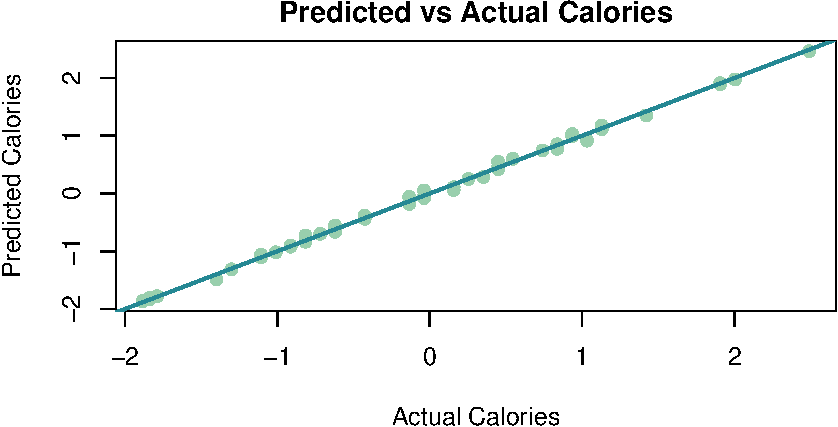
\includegraphics{Statistical_Learning_Final_Report_files/figure-latex/accuracy_lm-1} \end{center}

The actual and predicted values are close to each other, so the model is
a good fit

\subsubsection{Logistic Regression}\label{logistic-regression-1}

We split the data into training and testing sets, fit the logistic
regression model using the training set.

\begin{Shaded}
\begin{Highlighting}[]
\CommentTok{\# Fit the logistic regression model using the training set}
\NormalTok{glm\_model\_train }\OtherTok{\textless{}{-}} \FunctionTok{glm}\NormalTok{(y\_train }\SpecialCharTok{\textasciitilde{}}\NormalTok{ ., }\AttributeTok{data =}\NormalTok{ train\_data, }\AttributeTok{family =} \StringTok{"gaussian"}\NormalTok{)}
\FunctionTok{summary}\NormalTok{(glm\_model\_train)}
\end{Highlighting}
\end{Shaded}

\begin{verbatim}
## 
## Call:
## glm(formula = y_train ~ ., family = "gaussian", data = train_data)
## 
## Coefficients:
##                      Estimate Std. Error t value Pr(>|t|)    
## (Intercept)          0.384009   1.086638   0.353 0.724213    
## Total_Fat           11.010780   0.584930  18.824  < 2e-16 ***
## Trans_Fat           -2.384286   0.926402  -2.574 0.010876 *  
## Saturated_Fat       -6.394565  19.670475  -0.325 0.745499    
## Sodium              -0.344189   0.189423  -1.817 0.070894 .  
## Total_Carbohydrates  0.018919   0.008550   2.213 0.028182 *  
## Cholesterol          2.688521   0.393449   6.833 1.27e-10 ***
## Dietary_Fibre        1.334079   1.068310   1.249 0.213387    
## Sugars               1.270177   0.402629   3.155 0.001886 ** 
## Protein              2.288347   0.598184   3.825 0.000180 ***
## Vitamin_A            0.153517   0.104811   1.465 0.144767    
## Vitamin_C            0.192040   0.055413   3.466 0.000663 ***
## Calcium              0.458855   0.163646   2.804 0.005609 ** 
## Iron                -0.571726   0.080401  -7.111 2.70e-11 ***
## Caffeine             0.016253   0.006917   2.350 0.019895 *  
## ---
## Signif. codes:  0 '***' 0.001 '**' 0.01 '*' 0.05 '.' 0.1 ' ' 1
## 
## (Dispersion parameter for gaussian family taken to be 26.70325)
## 
##     Null deviance: 1896791.9  on 192  degrees of freedom
## Residual deviance:    4753.2  on 178  degrees of freedom
## AIC: 1198.1
## 
## Number of Fisher Scoring iterations: 2
\end{verbatim}

\begin{Shaded}
\begin{Highlighting}[]
\FunctionTok{AIC}\NormalTok{(glm\_model\_train)}
\end{Highlighting}
\end{Shaded}

\begin{verbatim}
## [1] 1198.059
\end{verbatim}

\begin{Shaded}
\begin{Highlighting}[]
\FunctionTok{BIC}\NormalTok{(glm\_model\_train)}
\end{Highlighting}
\end{Shaded}

\begin{verbatim}
## [1] 1250.262
\end{verbatim}

\paragraph{Model Evaluation}\label{model-evaluation-1}

We evaluate the model using the testing set. We make predictions using
the testing set and calculate the mean squared error and the root mean
squared error to assess the model's accuracy. We also plot the residuals
to check if the model is a good fit.

\begin{Shaded}
\begin{Highlighting}[]
\CommentTok{\# Make predictions using the testing set}
\NormalTok{predictions\_glm }\OtherTok{\textless{}{-}} \FunctionTok{predict}\NormalTok{(glm\_model\_train, }\AttributeTok{newdata =}\NormalTok{ test\_data)}

\CommentTok{\# Evaluate the model using the testing set}

\CommentTok{\# Calculate the mean squared error}
\NormalTok{mse\_glm }\OtherTok{\textless{}{-}} \FunctionTok{mean}\NormalTok{((y\_test }\SpecialCharTok{{-}}\NormalTok{ predictions\_glm)}\SpecialCharTok{\^{}}\DecValTok{2}\NormalTok{)}
\NormalTok{mse\_glm}
\end{Highlighting}
\end{Shaded}

\begin{verbatim}
## [1] 27.00986
\end{verbatim}

\begin{Shaded}
\begin{Highlighting}[]
\CommentTok{\# Calculate the root mean squared error}
\NormalTok{rmse\_glm }\OtherTok{\textless{}{-}} \FunctionTok{sqrt}\NormalTok{(mse\_glm)}
\NormalTok{rmse\_glm}
\end{Highlighting}
\end{Shaded}

\begin{verbatim}
## [1] 5.197101
\end{verbatim}

\begin{Shaded}
\begin{Highlighting}[]
\CommentTok{\# Now we plot the residuals to check if the model is a good fit}
\FunctionTok{par}\NormalTok{(}\AttributeTok{mfrow =} \FunctionTok{c}\NormalTok{(}\DecValTok{1}\NormalTok{, }\DecValTok{1}\NormalTok{))}
\FunctionTok{plot}\NormalTok{(glm\_model\_train, }\AttributeTok{which =} \DecValTok{1}\NormalTok{)}
\end{Highlighting}
\end{Shaded}

\begin{center}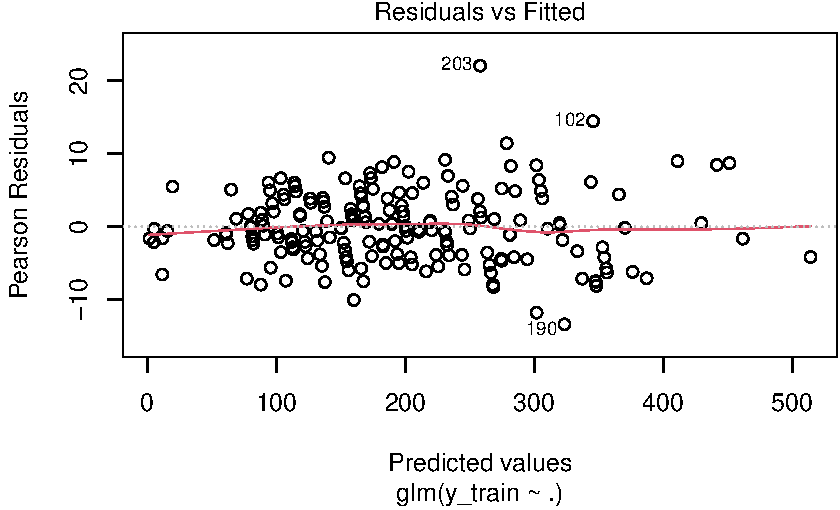
\includegraphics{Statistical_Learning_Final_Report_files/figure-latex/model_evaluation_glm-1} \end{center}

The residuals are randomly distributed around zero, so the model is a
good fit

Now we compute the accuracy of the model and then we plot the results

\begin{Shaded}
\begin{Highlighting}[]
\CommentTok{\# Compute the accuracy of the model}
\NormalTok{accuracy\_glm }\OtherTok{\textless{}{-}} \DecValTok{1} \SpecialCharTok{{-}}\NormalTok{ (rmse\_glm }\SpecialCharTok{/} \FunctionTok{mean}\NormalTok{(y\_test))}
\NormalTok{accuracy\_glm}
\end{Highlighting}
\end{Shaded}

\begin{verbatim}
## [1] 0.972211
\end{verbatim}

\begin{Shaded}
\begin{Highlighting}[]
\CommentTok{\# Plot the results}
\FunctionTok{plot}\NormalTok{(y\_test, predictions\_glm, }\AttributeTok{main =} \StringTok{"Actual vs Predicted Values"}\NormalTok{,}
     \AttributeTok{xlab =} \StringTok{"Actual Values"}\NormalTok{, }\AttributeTok{ylab =} \StringTok{"Predicted Values"}\NormalTok{,}
     \AttributeTok{col =} \StringTok{"\#ff810f"}\NormalTok{, }\AttributeTok{pch =} \DecValTok{19}\NormalTok{)}
\end{Highlighting}
\end{Shaded}

\begin{center}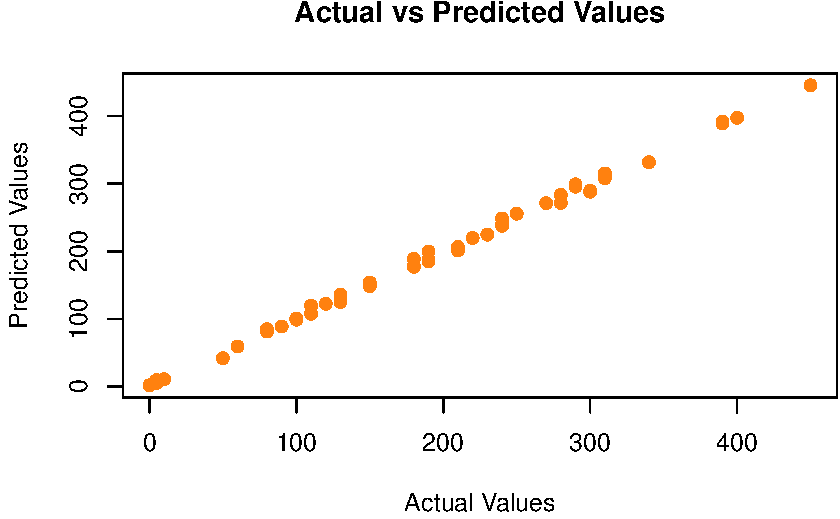
\includegraphics{Statistical_Learning_Final_Report_files/figure-latex/accuracy_glm-1} \end{center}

The actual and predicted values are close to each other, so the model is
a good fit

\end{document}
